%!TEX TS-program = xelatex
\documentclass[12pt]{article}
\usepackage{geometry}
\geometry{verbose,letterpaper,tmargin=2.2cm,bmargin=2.2cm,lmargin=2.2cm,rmargin=2.2cm}
\usepackage[doublespacing]{setspace}
\usepackage[left]{lineno}
\renewcommand{\linenumberfont}{\normalfont\tiny}

% Figures at the end of the manuscript

% fonts
\usepackage{lmodern}

% authors and affiliations
\usepackage{authblk}
\renewcommand\Authfont{\scshape\normalsize}
\renewcommand\Affilfont{\itshape\small}

\usepackage{amssymb,amsmath}
\usepackage{ifxetex,ifluatex}
\ifnum 0\ifxetex 1\fi\ifluatex 1\fi=0 % if pdftex
  \usepackage[T1]{fontenc}
  \usepackage[utf8]{inputenc}
  \usepackage{textcomp} % provide euro and other symbols
\else % if luatex or xetex
  \usepackage{unicode-math}
  \defaultfontfeatures{Scale=MatchLowercase}
  \defaultfontfeatures[\rmfamily]{Ligatures=TeX,Scale=1}
\fi

% Use upquote if available, for straight quotes in verbatim environments
\IfFileExists{upquote.sty}{\usepackage{upquote}}{}
\IfFileExists{microtype.sty}{% use microtype if available
  \usepackage[]{microtype}
  \UseMicrotypeSet[protrusion]{basicmath} % disable protrusion for tt fonts
}{}
\makeatletter
\@ifundefined{KOMAClassName}{% if non-KOMA class
  \IfFileExists{parskip.sty}{%
    \usepackage{parskip}
  }{% else
    \setlength{\parindent}{0pt}
    \setlength{\parskip}{6pt plus 2pt minus 1pt}}
}{% if KOMA class
  \KOMAoptions{parskip=half}}
\makeatother
\usepackage{xcolor}
\IfFileExists{xurl.sty}{\usepackage{xurl}}{} % add URL line breaks if available
\IfFileExists{bookmark.sty}{\usepackage{bookmark}}{\usepackage{hyperref}}
\hypersetup{
  pdftitle={Spatial Structure is More Than Habitat Amount: A Metapopulation Approach is Necessary to Project Distributions Under Climate Change},
  pdfauthor={Victor~Cameron and F.
Guillaume~Blanchet and Yan~Boulanger and Junior
A.~Tremblay and Dominique~Gravel},
  pdflang={en},
  pdfkeywords={Climate change, Metapopulation theory, Species
distribution, Range shift, Transient dynamics},
colorlinks=true,
allcolors=[rgb]{0,0.4,0.5},
pdfcreator={LaTeX via pandoc}}
\urlstyle{same} % disable monospaced font for URLs






\usepackage{graphicx}
\makeatletter
\def\maxwidth{\ifdim\Gin@nat@width>\linewidth\linewidth\else\Gin@nat@width\fi}
\def\maxheight{\ifdim\Gin@nat@height>\textheight\textheight\else\Gin@nat@height\fi}
\makeatother
% Scale images if necessary, so that they will not overflow the page
% margins by default, and it is still possible to overwrite the defaults
% using explicit options in \includegraphics[width, height, ...]{}
\setkeys{Gin}{width=\maxwidth,height=\maxheight,keepaspectratio}
% Set default figure placement to htbp
\makeatletter
\def\fps@figure{htbp}
\makeatother


\setlength{\emergencystretch}{3em} % prevent overfull lines
\providecommand{\tightlist}{%
  \setlength{\itemsep}{0pt}\setlength{\parskip}{0pt}}

\setcounter{secnumdepth}{5}




\newlength{\cslhangindent}
\setlength{\cslhangindent}{1.5em}
\newenvironment{cslreferences}%
  {\setlength{\parindent}{0pt}%
  \everypar{\setlength{\hangindent}{\cslhangindent}}\ignorespaces}%
  {\par}


% MAKETITLE: print all title page only if not double-blind
\title{Spatial Structure is More Than Habitat Amount: A Metapopulation
Approach is Necessary to Project Distributions Under Climate Change}

\date{}

\linenumbers

\begin{document}

% print all title page only if not double-blind
\maketitle
\begin{abstract}
Projecting species distributions under climate change requires going
beyond climate suitability models. We propose that metapopulation theory
can be used to leverage species distribution models while accounting for
landscape spatial structure, biotic interactions and demography. While
reviewing how metapopulation theory reacts to climate-induced
distribution shifts, we found that habitat-climate mismatch can generate
non-equilibrium dynamics, linear change in habitat occupancy generates
non-linear distribution change, and the effect of environmental change
on habitat can have counterintuitive effects on higher trophic levels.
We illustrated our findings by developing habitat suitability models for
the Bicknell's Thrush (\emph{Catharus bicknelli}) a red-listed bird
species confined to perturbed balsam fir forests. Under climate warming,
the Bicknell's Thrush distribution shifts northwards from the effect of
climate alone while the distribution of its associated vegetation
remains stable despite warming. The arising mismatch between climate and
vegetation changes patch size, connectivity, and habitat structure
potentially to different extent, influencing species persistence and
suggesting that habitat alone is not enough to characterize regional
distribution changes. Our results emphasize the importance of both
habitat and landscape spatial structure in assessing persistence for
which metapopulation theory is an ideal framework to further advance our
understanding of species distribution.
\end{abstract}
\newpage



\hypertarget{introduction}{%
\section{Introduction}\label{introduction}}

Climate change has already prompted species to shift their range toward
higher latitudes and elevations (Chen et al.
\protect\hyperlink{ref-chen_rapid_2011}{2011}, Parmesan
\protect\hyperlink{ref-parmesan_ecological_2006}{2006}, Virkkala and
Lehikoinen \protect\hyperlink{ref-virkkala_patterns_2014}{2014}).
Species persistence in response to climate change may critically depend
on their ability to expand their range and track suitable environments.
While most current predictive approaches ignore important biological
mechanisms such as demography, dispersal, and biotic interactions, these
play key roles in species response to environmental change (Urban et al.
\protect\hyperlink{ref-urban_improving_2016}{2016}). In response,
several calls have been made for models to incorporate the processes
mediating species response (Fordham et al.
\protect\hyperlink{ref-fordham_adapted_2013}{2013}, Stralberg et al.
\protect\hyperlink{ref-stralberg_conservation_2015}{2015},
\protect\hyperlink{ref-stralberg_conservation_2019}{2019}) and
mechanistic approaches have been developed to improve the realism of
projections. However, more work is required to increase accuracy and
usability of mechanistic models as they remain rarely employed in
conservation planning when compared to correlative species distribution
models (SDMs, Guisan and Thuiller
\protect\hyperlink{ref-guisan_predicting_2005}{2005}, Franklin and
Miller \protect\hyperlink{ref-franklin_mapping_2009}{2009}, Guisan et
al. \protect\hyperlink{ref-guisan_predicting_2013}{2013}). The challenge
now lies in the development of approaches that are accessible,
customizable and integrate multiple processes and their interplay
(McIntire et al. \protect\hyperlink{ref-mcintire_perfict_2022}{2022},
Thuiller et al. \protect\hyperlink{ref-thuiller_road_2013}{2013}, Urban
et al. \protect\hyperlink{ref-urban_improving_2016}{2016}).

Explicit modelling of the processes that underlie distribution dynamics
is challenging (Briscoe et al.
\protect\hyperlink{ref-briscoe_can_2021}{2021}, Hefley et al.
\protect\hyperlink{ref-hefley_when_2017}{2017}). Dynamic range models
provide a successful example of incorporating demographic processes and
dispersal to improve the accuracy of species distribution projections
(Briscoe et al. \protect\hyperlink{ref-briscoe_can_2021}{2021}). They
are based on niche theory, assuming that species occur at locations
where the environment allows positive growth rates (Godsoe et al.
\protect\hyperlink{ref-godsoe_integrating_2017}{2017}, Hutchinson
\protect\hyperlink{ref-hutchinson_concluding_1957}{1957}). However, such
models are often difficult to parameterize because measuring growth rate
is challenging (McGill \protect\hyperlink{ref-mcgill_trees_2012}{2012})
and requires very specific data on species response to abiotic
environmental conditions. Indeed, on top of being computationally
intensive (Snell et al. \protect\hyperlink{ref-snell_using_2014}{2014}),
the data required to parameterize these models are rarely available
(Urban et al. \protect\hyperlink{ref-urban_improving_2016}{2016}).
Furthermore, local demography on its own may be insufficient to explain
broad-scale species distribution, suggesting that processes at broader
scales must also be considered (Le Squin et al.
\protect\hyperlink{ref-le_squin_climateinduced_2021}{2021}), including
dispersal limitations, disturbances, and biotic interactions (Stephan et
al. \protect\hyperlink{ref-stephan_positive_2021}{2021}, Urban et al.
\protect\hyperlink{ref-urban_improving_2016}{2016}).

Another approach recently proposed is derived from metapopulation
theory. Metapopulations are expected to persist in heterogenous
landscapes if colonization is sufficient to balance local extinctions
(Hanski and Ovaskainen
\protect\hyperlink{ref-hanski_metapopulation_2000}{2000}). The
environment may constrain these two processes and limit metapopulation
persistence. Distribution limits eventually emerge over environmental
gradients at this location where persistence becomes critical.
Furthermore, distributions may be constrained by the amount of suitable
conditions in a region. As a result, a species may be absent from a
region, or a portion of a gradient, despite the occurrence of suitable
conditions if these are not abundant enough or if extinction is too
high. Metapopulation theory also makes an ideal framework to incorporate
several elements of complexity such as landscape heterogeneity,
dispersal, and biotic interactions as it is flexible enough to integrate
fundamental processes driving distribution dynamics.

Disturbances, environmental changes, and biotic interactions are
processes that may cause species distribution to be constantly out of
equilibrium with their niche (Boulangeat et al.
\protect\hyperlink{ref-boulangeat_transient_2018}{2018}, Ovaskainen and
Hanski \protect\hyperlink{ref-ovaskainen_transient_2002}{2002}, Svenning
et al. \protect\hyperlink{ref-svenning_influence_2014}{2014}).
Non-equilibrium dynamics are especially marked in plants that are
limited by slow demography and restricted dispersal (Savage and Vellend
\protect\hyperlink{ref-savage_elevational_2015}{2015}, Svenning and
Sandel \protect\hyperlink{ref-svenning_disequilibrium_2013}{2013},
Vissault et al. \protect\hyperlink{ref-vissault_slow_2020}{2020}).
Representing this reality requires an adapted approach and
metapopulation theory offers the opportunity to model non-equilibrium
dynamics (Hanski and Simberloff
\protect\hyperlink{ref-hanski_metapopulation_1997}{1997}, Ovaskainen and
Hanski \protect\hyperlink{ref-ovaskainen_transient_2002}{2002}).
Metapopulation models have shown the trailing edge of current tree
distribution to be persisting despite unfavourable climatic conditions
as slow demography delays the extinction of populations. At the leading
edge, dispersal limitations and competition prevent trees from
colonizing favourable habitats (Talluto et al.
\protect\hyperlink{ref-talluto_extinction_2017}{2017}). The ability of
metapopulation models to study and describe dynamic landscapes therefore
makes them particularly suitable to study persistence under changing
climate.

In this paper, we show how metapopulation theory can be used to model
and thus complement the interpretation of species distribution in a
changing environment. In addition, we illustrate how metapopulation
theory can be used to leverage species distribution models by accounting
for the complexity arising from biotic interactions, demography, and
landscape structure. After reviewing the theory to account for these key
ecological processes in distribution modelling and present associated
sources of complexity, we illustrate the effect and importance of these
processes on persistence and distribution dynamics using the Bicknell's
Thrush (\emph{Catharus bicknelli}), a red-listed bird species, as a case
study (IUCN \protect\hyperlink{ref-iucn_catharus_2020}{2020}).

\hypertarget{key-concepts-arising-from-metapopulation-theory}{%
\section{Key Concepts Arising From Metapopulation
Theory}\label{key-concepts-arising-from-metapopulation-theory}}

\hypertarget{model-description}{%
\subsection{Model description}\label{model-description}}

The classic metapopulation model describes species distribution over a
set of suitable patches of habitat connected by dispersal (Levins
\protect\hyperlink{ref-levins_mathematical_1970}{1970},
\protect\hyperlink{ref-levins_demographic_1969}{1969}). Regional
dynamics are driven by colonization and extinction events, which
corresponding rates depend on local environmental conditions. Together
they define the species distribution limits. The dynamics may be
complexified with the representation of several trophic levels, where
high-trophic level species occur exclusively at locations occupied by
lower-level species (Fordham et al.
\protect\hyperlink{ref-fordham_adapted_2013}{2013}). We adopt the
specialist-habitat terminology throughout this study to lighten the text
and fit the example, even if the results are more general and can apply
to any bottom-up system (e.g., predator-prey or host-mutualist).

Consider a simplistic system composed of a specialist species tracking
the spatial distribution of a dynamic favourable habitat, such as a
particular type of vegetation patch providing shelter and food. The
model represents the dynamics of the occupancy of three possible states:
empty, occupied by the favourable habitat alone (\(H\)) or in
co-occurrence with the specialist (\(S\)). The landscape is
heterogeneous and each local patch is characterized by the abiotic
environmental condition (\(E\)). Dynamics of occupancy are given by the
following system of differential equations:

\[
\frac{dH(E)}{dt} = c_{H}(E)H(1-H) - e_{H}(E)H
\]

\[
\frac{dS(E)}{dt} = c_{S}(E)S(H(E)-S) - e_{S}(E)S
\]

Where \(c(E)\) is the function for colonization rate and \(e(E)\) for
the extinction rate. Both are species-specific functions of the abiotic
environment such that \(H\) and \(S\) also depend on \(E\), the abiotic
environmental conditions. A specialist persists over the landscape in a
dynamic equilibrium between habitat availability (i.e., habitat
occupancy over the landscape), colonization, and extinction if its
occupancy \(S\) is larger than zero:

\[
S(E^{*}) = H(E^{*}) - \frac{e_{S}(E^{*})}{c_{S}(E^{*})}
\]

and the distribution limit is defined by \(S(E^{*}) = 0\), such that it
is located where \(H(E^{*}) = \frac{e_{S}(E^{*})}{c_{S}(E^{*})}\).
Distribution limits of a habitat specialist are therefore determined by
its intrinsic response to the abiotic environment (the ratio
\(\frac{e_{S}(E)}{c_{S}(E)}\)), in conjunction with the habitat response
to the abiotic environment (\(\frac{e_{H}(E)}{c_{H}(E)}\)).

\hypertarget{graphical-representation-of-range-limits}{%
\subsection{Graphical representation of range
limits}\label{graphical-representation-of-range-limits}}

We provide three examples to illustrate how metapopulation theory can
reveal some of the complexities of distribution dynamics under a
changing climate.

A specialist's persistence and therefore occupancy is jointly affected
by environmental conditions and habitat availability (occupancy) such
that it can be represented graphically with \(\frac{e(E)}{c(E)}\) and
\(H(E)\) curves (Figure \ref{fig:occ_plot}). Distribution limit occurs
at the position along the environmental gradient where the habitat
occupancy curve crosses the extinction to colonization ratio. The
specialist's occupancy for given environmental conditions is defined by
the difference between habitat availability and the extinction to
colonization ratio curves (\(S^{*} = H-\frac{e}{c}\)). The difference
between habitat availability and the extinction to colonization ratio
curves (\(S^{*}\); shown by the arrows in Figure \ref{fig:occ_plot} A)
is reduced with increasing environmental conditions, illustrating a
decrease in the specialist's occupancy and persistence
(\(S(E_{0}^{*}) > S(E_{1}^{*})\)).

\hypertarget{interaction-of-the-specialist-and-of-its-habitats-response-can-cause-indirect-distribution-dynamics}{%
\subsubsection{Interaction of the specialist and of its habitat's
response can cause indirect distribution
dynamics}\label{interaction-of-the-specialist-and-of-its-habitats-response-can-cause-indirect-distribution-dynamics}}

\begin{figure}
\hypertarget{fig:occ_plot}{%
\centering
\includegraphics[width=1\textwidth,height=\textheight]{./manuscript/img/concept_occ.png}
\caption{Change in occupancy (and persistence as shown by the grey
arrows) of the habitat specialist depends on its intrinsic response to
the environment \(\frac{e}{c}\) (orange line) and of the habitat's
occupancy \(H(E^{*})\) (green line).}\label{fig:occ_plot}
}
\end{figure}

In a bottom-up system such as predator-prey or a habitat specialist, the
response to environmental change does not only depend on the focal
species but also on the response of the associated one. The covariation
in the response to the environment between the two levels is therefore
of critical importance. For instance, the net effect of less favourable
environmental conditions to a specialist could be detrimental (Figure
\ref{fig:occ_plot} A), without effect (Figure \ref{fig:occ_plot} B), or
favourable (Figure \ref{fig:occ_plot} C) depending on the effect of the
environment to its habitat. Thus, the interaction between trophic levels
may have indirect (and counterintuitive) effects on specialist response.

\hypertarget{habitat-mismatch-affects-species-distribution-shifts}{%
\subsubsection{Habitat mismatch affects species distribution
shifts}\label{habitat-mismatch-affects-species-distribution-shifts}}

\begin{figure}
\hypertarget{fig:concept_mismatch}{%
\centering
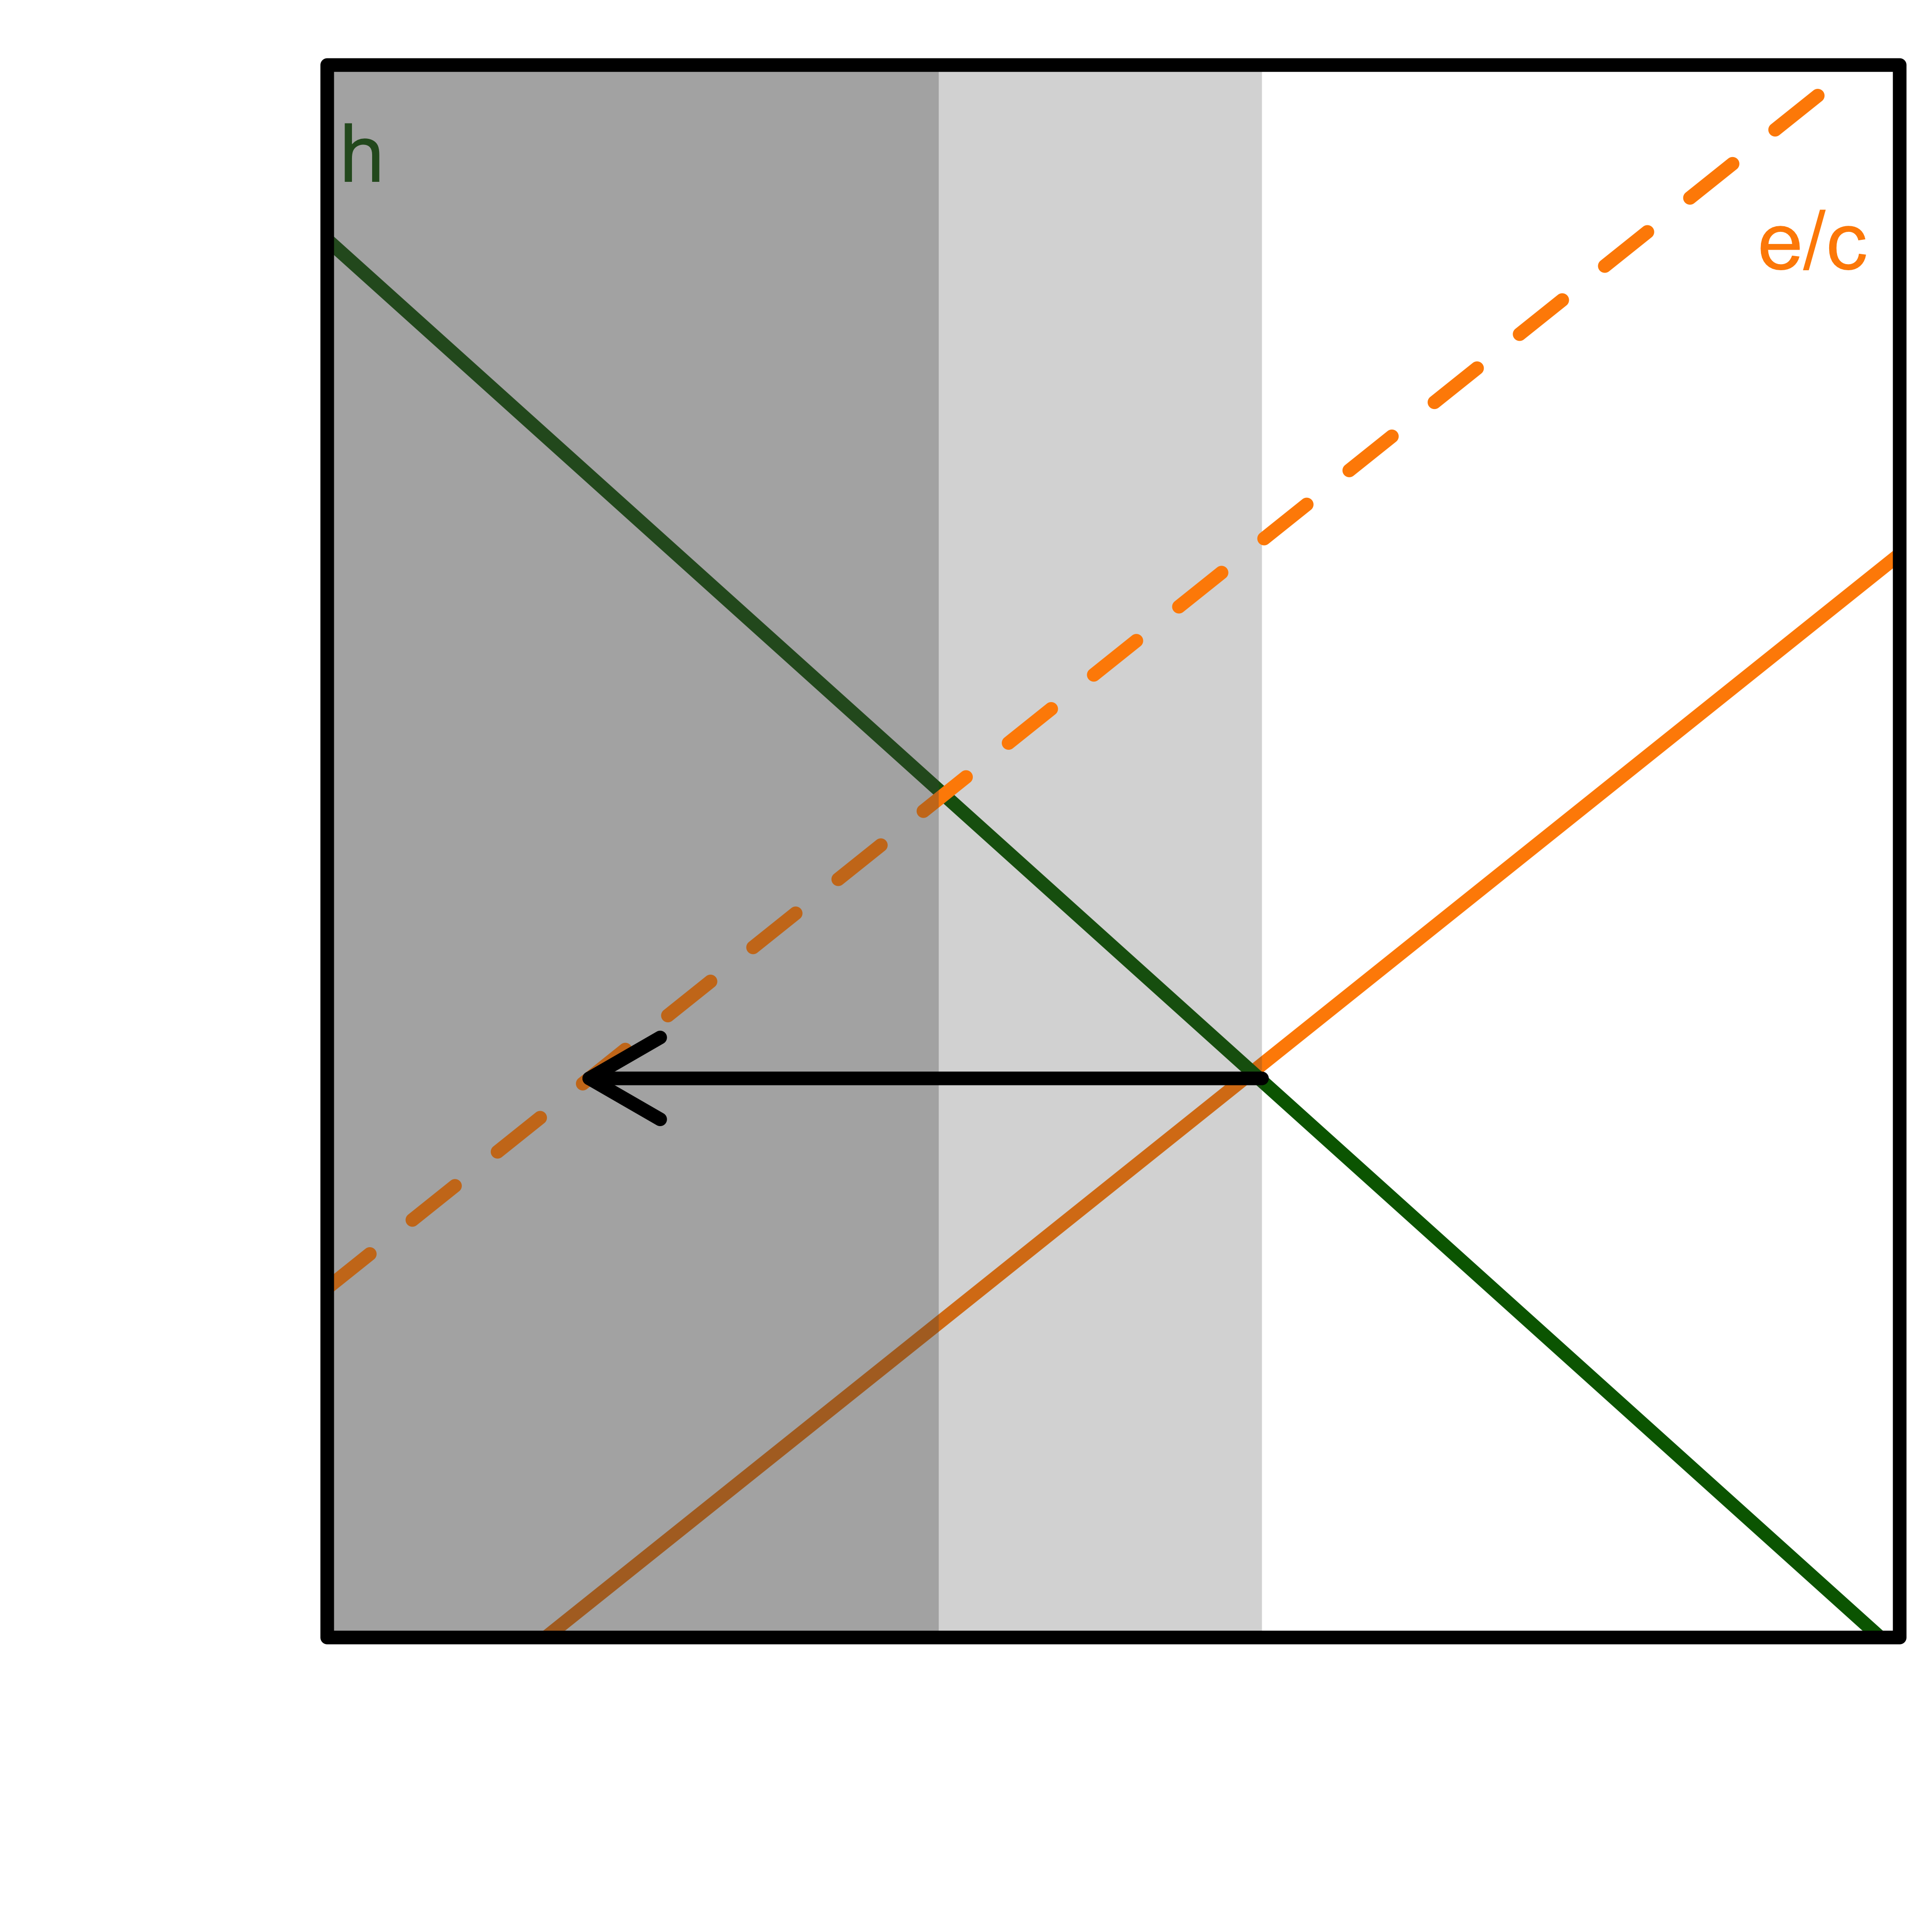
\includegraphics[width=0.35\textwidth,height=\textheight]{./manuscript/img/concept_mismatch.png}
\caption{The distribution of the habitat specialist (grey area) is
impacted by the functions relating the intrinsic response to the
environment (orange line) to habitat occupancy (\(H(E)\), full and
dashed green lines). A change in the habitat occupancy at given
environmental conditions (full to dashed green line) affects the
specialist's persistence and shifts its distribution on the
environmental gradient (dark to light grey
area).}\label{fig:concept_mismatch}
}
\end{figure}

Range limits of a habitat specialist is jointly affected by
environmental conditions and the availability (occupancy) of its
habitat. Range shift in response to environmental changes is therefore
not only determined by its intrinsic response to the environment, but
also by the response of the habitat to the environment. As a result, a
mismatch between the species response to the environment and its
realized distribution may arise, in particular when different trophic
levels are not responding at the same rate to environmental change
(Figure \ref{fig:concept_mismatch}). The distribution may shift in the
geographic space, for instance toward the north, but it should stay the
same in the environmental space if both levels respond similarly (Figure
\ref{fig:concept_mismatch}, dark shaded area). That said, if a delay or
any other factor prevents the habitat from tracking the new
environmental conditions, then the habitat curve will shift (Figure
\ref{fig:concept_mismatch}, green dashed line), and so will the
distribution limit (light shaded area). Such mismatch could either
benefit or harm the specialist distribution; in Figure
\ref{fig:concept_mismatch}, the specialist expands to less favourable
environmental conditions. The response of the habitat to changing
environmental conditions does influence the specialist distribution,
both in extent and in the position of its distribution limits in
environmental and geographical space.

\hypertarget{metapopulation-dynamics-may-precipitate-species-decline}{%
\subsubsection{Metapopulation dynamics may precipitate species
decline}\label{metapopulation-dynamics-may-precipitate-species-decline}}

\begin{figure}
\hypertarget{fig:concept_metapop}{%
\centering

\includegraphics[width=0.35\textwidth,height=\textheight]{./manuscript/img/concept_metapopEffect.png}
\caption{The response of a habitat specialist to a linear environmental
change in time as it would be expected with a correlative SDM (linear
response; full line). Metapopulation dynamics may precipitate - or
alternatively delay - the extinction of the species in a metapopulation
even if there are suitable conditions (dashed
line).}\label{fig:concept_metapop}
}
\end{figure}

The projection of range shifts with correlative SDMs assumes an
instantaneous response to environmental change. An implicit assumption
is also that a reduction in habitat occupancy translates into an
equivalent reduction in the specialist's range, leading to extinction
(Thomas et al. \protect\hyperlink{ref-thomas_extinction_2004}{2004}).
Metapopulation dynamics may, however, precipitate the decline of a
species before the complete disappearance of suitable conditions.
Consider a landscape where environmental conditions are spatially
heterogeneous, such as temperature in a mountainous area. The
progressive change in this environment, like climate warming, will have
two effects on the distribution of suitable patches: the first direct
consequence is a reduction in habitat occupancy \(H(E)\), and indirectly
follows the increase of the extinction rate with the shrinking of
suitable patches. Some favourable patches may also disappear, thereby
reducing the landscape connectivity. A non-linear decline of occupancy
therefore arises from a linear change in environmental conditions as the
ratio \(\frac{e(E)}{c(E)}\) within the specialist's persistence function
increases (Figure \ref{fig:concept_metapop}). This metapopulation effect
may not be important at first while suitable habitat is abundant and
patches are large, but increases as habitat occupancy decreases,
supporting an acceleration of metapopulation prevalence loss to a
constant environmental environmental shift (Hanski and Ovaskainen
\protect\hyperlink{ref-hanski_metapopulation_2000}{2000}, Ovaskainen and
Hanski \protect\hyperlink{ref-ovaskainen_transient_2002}{2002}).

\hypertarget{spatially-explicit-landscapes}{%
\subsection{Spatially explicit
landscapes}\label{spatially-explicit-landscapes}}

Analytical tools from metapopulation theory can be used to interpret
range limits in spatially explicit heterogeneous landscapes.
Metapopulation capacity can be evaluated for realistic landscapes where
patch coordinates and size are considered. Metapopulation capacity is
measured as the first eigenvalue of the landscape matrix \(M\), where
elements \(m_{ij} = exp(-\alpha d_{ij})A_{i}A_{j}\) for \(j \neq i\) and
\(m_{ii} = 0\) (Hanski and Ovaskainen
\protect\hyperlink{ref-hanski_metapopulation_2000}{2000}).
\(\frac{1}{\alpha}\) describes the average dispersal distance,
\(d_{ij}\) is the distance between patch \(i\) and \(j\), and \(A_{i}\)
is the area of patch \(i\) (refer to Hanski and Ovaskainen
(\protect\hyperlink{ref-hanski_metapopulation_2000}{2000}) for the full
description). Metapopulation capacity is a measure of a species' ability
to maintain itself regionally as a function of connectivity and local
extinctions. It provides the means to evaluate conditions for
persistence given the spatial arrangement of patches and their size.

Climate change can profoundly alter landscapes as experienced by
species; not only does it influence the amount of suitable habitats, but
also the capacity of species to persist when colonization and extinction
prevail. Consider a mountainous landscape inhabited by a high elevation
habitat specialist. The landscape is marked by a steep elevational
gradient in temperature where warm temperatures at low elevations exceed
the species' tolerance. The landscape would therefore be divided between
suitable cold habitats on mountain tops and unsuitable warmer habitats
at the bottom. The topography will not only determine the total surface
of suitable conditions, but also the frequency distribution of patch
sizes and of distances among mountain tops. As a result, it will
influence the connectivity of the landscape and the distribution of
patch specific extinction rates.

A schematic example is provided in Figure
\ref{fig:concept_metapop_structure}, inspired by the case study that
will follow in the next section. Fixing a lower climatic range limit in
a hypothetical mountainous landscape, we find nine suitable habitat
patches of various sizes, distributed at various distances one from
another (Figure \ref{fig:concept_metapop_structure}, left panel).
Habitat patches here represent high elevation mountain tops. The warming
of climatic conditions causes an elevational shift of lower range limits
resulting in the contraction of habitat patches and a decline in the
number of patches (Figure \ref{fig:concept_metapop_structure}, right
panel). Patches become generally smaller from contraction and
fragmentation, and the smallest patches go extinct. Further, not only
smaller patches are assumed to support smaller population sizes, have
superior extinction risks, and produce fewer colonizers (Hanski and
Ovaskainen \protect\hyperlink{ref-hanski_metapopulation_2000}{2000}),
but the loss and the fragmentation of patches alter species dispersal
ability through the loss of connectivity (Huang et al.
\protect\hyperlink{ref-huang_using_2019}{2019}).

The decrease in metapopulation capacity surpasses that of habitat
amount, adding a spatial structure perspective to the assumptions made
by correlative approaches. The overall effect of climate warming is not
only to modify patch areas, but to change species' ability to colonize
and occupy these patches.

\begin{figure}
\hypertarget{fig:concept_metapop_structure}{%
\centering
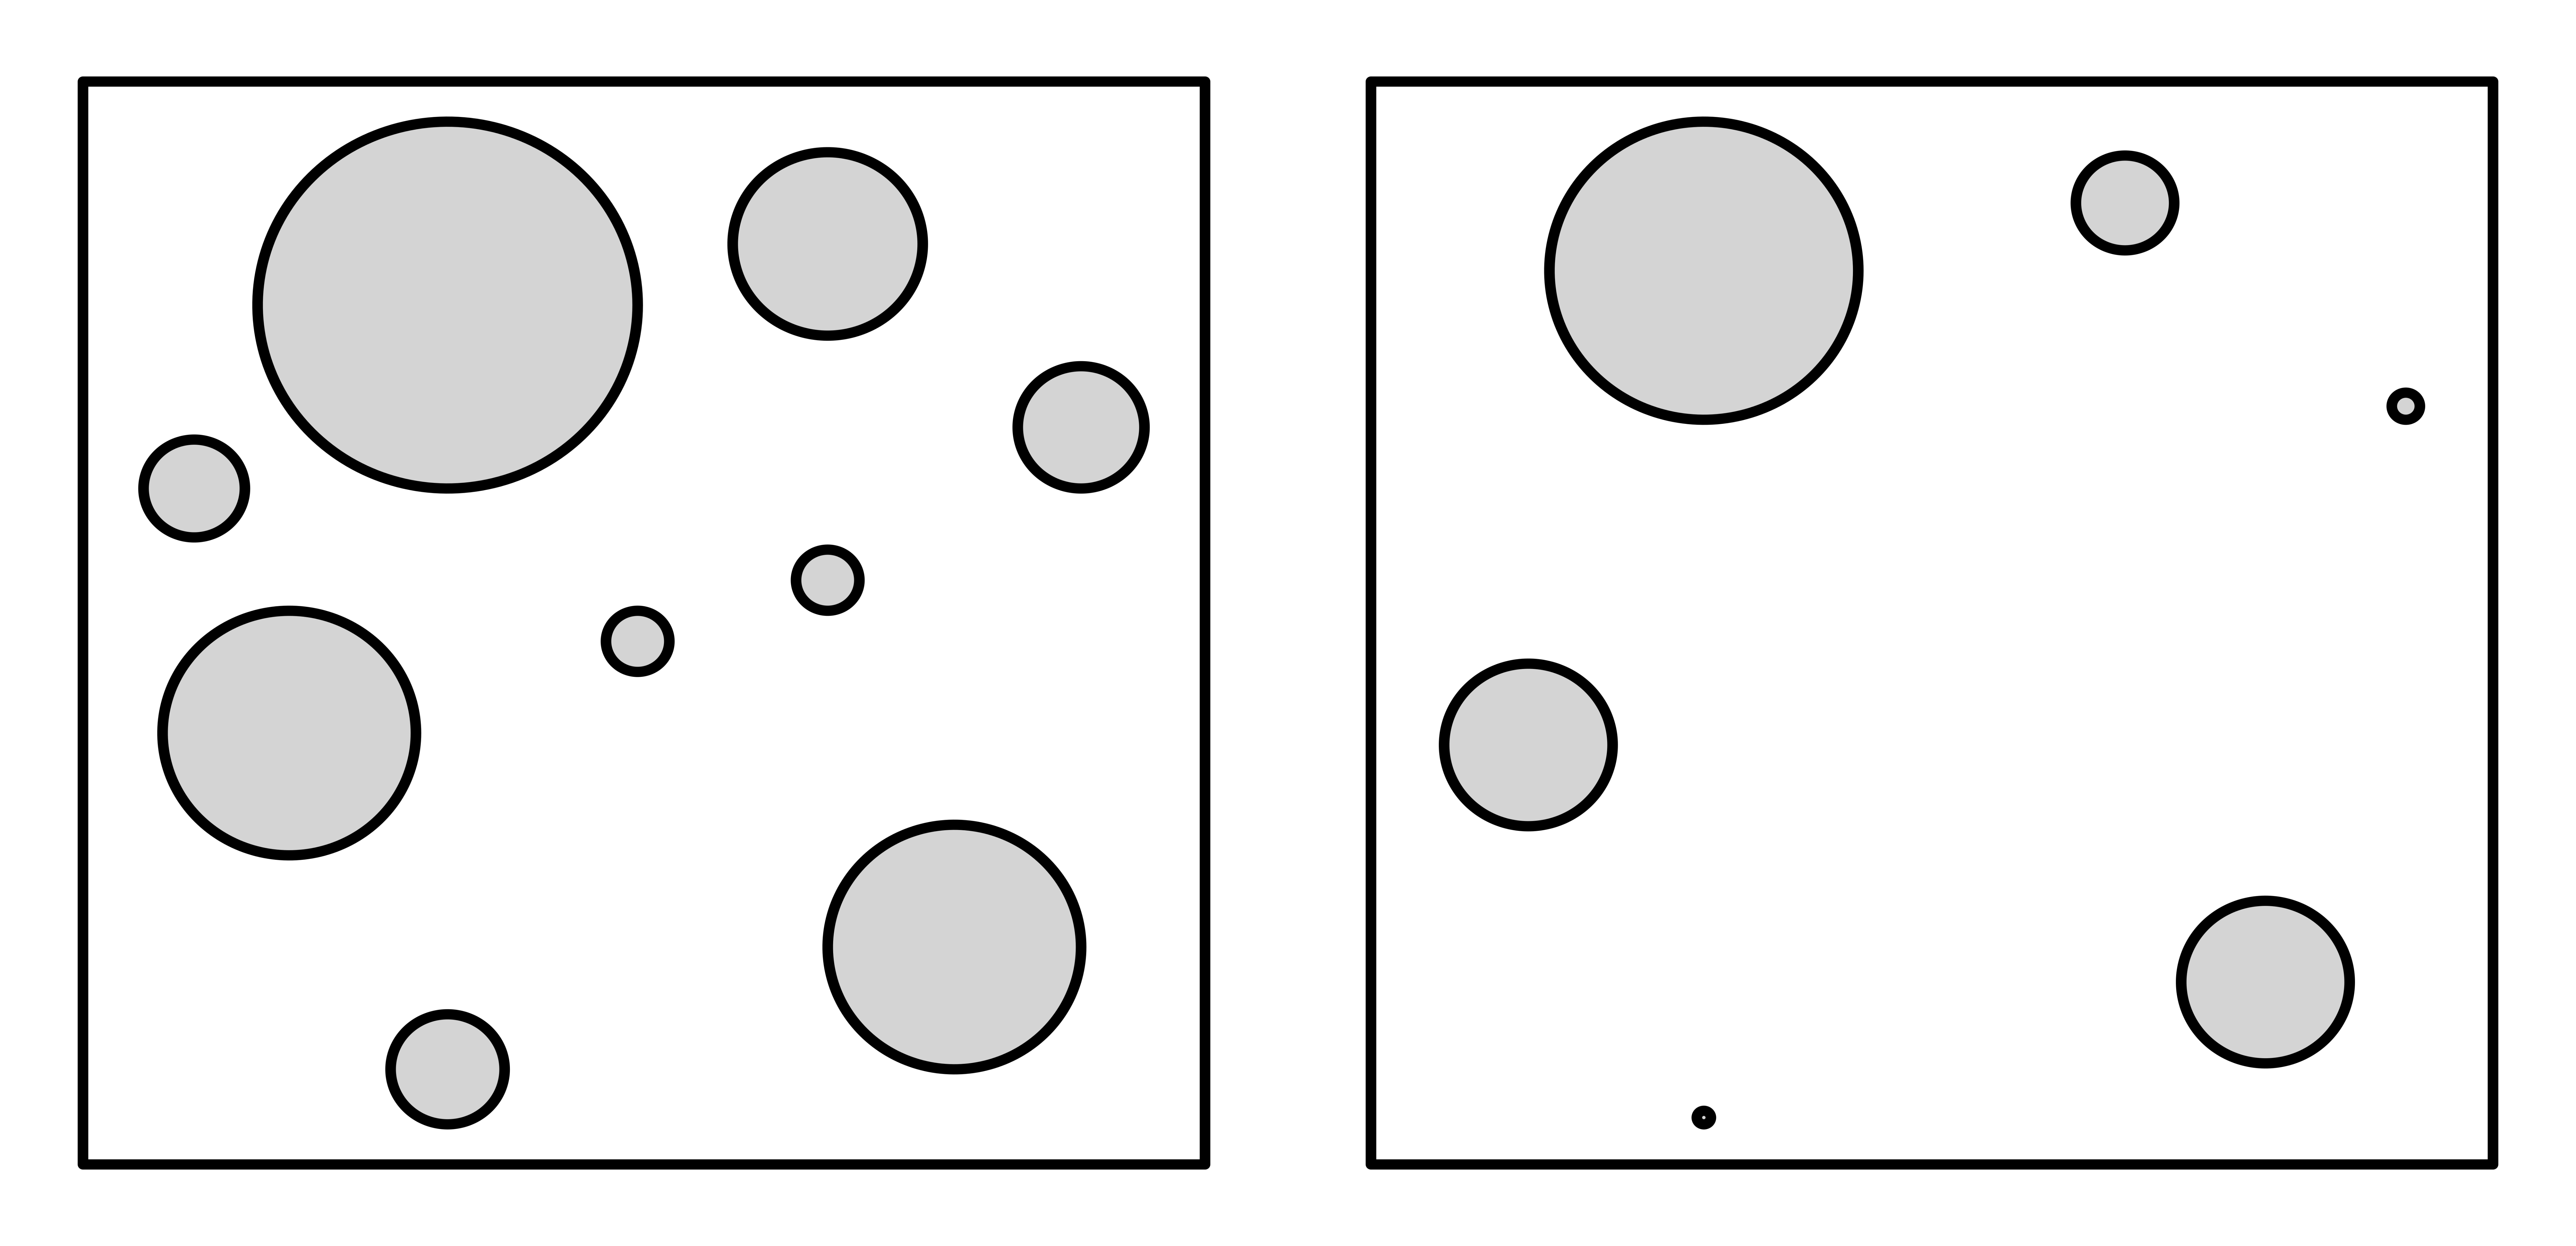
\includegraphics[width=0.7\textwidth,height=\textheight]{./manuscript/img/concept_metapop_structure.png}
\caption{Species persistence is affected by changes to landscape
connectivity as well as habitat amount. Circles delimit suitable habitat
patches. The left panel presents a hypothetical mountainous landscape
where suitable patches represent high elevation mountain tops. The right
panel illustrates the same landscape where patches's radius contracted
by an equal amount, simulating an elevation shift of climatic conditions
on landscape suitability. Following patch contraction, metapopulation
capacity declined by 82\% whereas habitat amount only declined by
63\%.}\label{fig:concept_metapop_structure}
}
\end{figure}

\hypertarget{case-study-bicknells-thrush-in-north-eastern-america}{%
\section{Case Study: Bicknell's Thrush in North-Eastern
America}\label{case-study-bicknells-thrush-in-north-eastern-america}}

We illustrate the concepts presented in the previous section with a case
study of the Bicknell's Thrush (\emph{Catharus bicknelli}), a threatened
bird species in Canada (COSEWIC
\protect\hyperlink{ref-cosewic_cosewic_2022}{2022}, IUCN
\protect\hyperlink{ref-iucn_catharus_2020}{2020}). Bicknell's Thrush is
the smallest Nordic thrush within the \emph{Catharus} genus and is
visually similar to the Grey-cheeked Thrush (\emph{Catharus minimus}).
It migrates in Northeastern North America from its wintering grounds in
the Greater Antilles and feeds on invertebrates and small fruits
(Townsend et al.
\protect\hyperlink{ref-billerman_bicknells_2020}{2020}). Populations are
small and were reported to be declining in Canada (COSEWIC
\protect\hyperlink{ref-cosewic_cosewic_2022}{2022}). The dispersal of
Bicknell's Thrush is not known with certainty, although it has been
suggested that adults nest near the site of previous successful nesting
while few yearlings are observed to come back to their site of birth
(Collins \protect\hyperlink{ref-collins_spatial_2007}{2007}, Rimmer et
al. \protect\hyperlink{ref-rimmer_bicknells_2001}{2001}, Studds et al.
\protect\hyperlink{ref-studds_stable-hydrogen_2012}{2012}). The
Bicknell's Thrush is known to be associated with very dense balsam fir
(\emph{Abies Balsamea}) forests, mostly at high elevations, resulting in
a fragmented and highly restricted range (Cadieux et al.
\protect\hyperlink{ref-cadieux_spatially_2019}{2019}, COSEWIC
\protect\hyperlink{ref-cosewic_cosewic_2022}{2022}). This habitat may be
ephemeral, as natural disturbances, forestry and stand succession could
lead to local extinctions. Furthermore, its distribution in mountainous
areas is highly contingent on climate elevation gradients. Climate
change could therefore pose a major threat to the persistence of this
species as favourable climatic conditions within isolated habitat
patches could shrink rapidly (Rodenhouse et al.
\protect\hyperlink{ref-rodenhouse_potential_2008}{2008}). Unfavourable
environmental conditions are predicted to increase at the edges of
mountaintop fir forest patches with the warming of climate and the
limited response capacity of boreal tree species (Talluto et al.
\protect\hyperlink{ref-talluto_extinction_2017}{2017}, Vissault et al.
\protect\hyperlink{ref-vissault_slow_2020}{2020}).

In the following section, we project the changes to the Bicknell's
Thrush breeding range in response to climate forcing using a standard
correlative approach. We then leverage the projections using the
concepts developed to analyze the total amount of favourable habitat,
the distribution of patch areas, their connectivity, and the
metapopulation capacity. Finally, we compare Bicknell's Thrush
favourable landscapes under climate-only change and climate-induced
forest change scenarios to illustrate arising climate-habitat mismatch.
Thereby, we wish to reveal the joint effects of these two components of
Bicknell's Thrush's distribution and demonstrate their importance on
distribution dynamics.

\hypertarget{methods}{%
\subsection{Methods}\label{methods}}

\hypertarget{studied-region}{%
\subsubsection{Studied region}\label{studied-region}}

The Bicknell's Thrush breeding range was projected for the province of
Québec where the majority of the Canadian occurrences are found,
specifically in the Appalachian Mountains in the southeast and the
Laurentians Mountains north of the St.~Lawrence River (COSEWIC
\protect\hyperlink{ref-cosewic_cosewic_2022}{2022}, Townsend et al.
\protect\hyperlink{ref-billerman_bicknells_2020}{2020}). The landscape
is composed of boreal, mixed and temperate forests, with their
distributions mainly driven by climatic latitudinal and elevational
gradients. Mean annual temperature ranges from -4.0 to 7.5 °C in this
region, but the Bicknell's Thrush occupies locations with a more
restricted range because of its preference for high-elevation areas.
Annual precipitation ranges from 730 to 950 mm.

\hypertarget{data}{%
\subsubsection{Data}\label{data}}

Distribution data consisted of 6,079 confirmed observations of nesting
behavior, with geographic precision to \textasciitilde30 m (1 second of
latitude/longitude), sampled from 1994 to 2020. Data were provided by
the Regroupement QuébecOiseaux (SOS-POP
\protect\hyperlink{ref-sos-pop_banque_2021}{2021}). It contains
observations from various sources, including scientific surveys and
citizen science. The region of interest was rasterized on a grid of 250
x 250 m cells, where an observation within a cell was defined as a
presence. We considered the locations where one or more observations
were made as a single presence, accounting for any potential effects of
temporal and spatial pseudo-replication resulting, for example, from
multiple sightings of the one individual in the same location.

Mean annual temperature, total annual precipitation, elevation, and
balsam fir biomass were used to model occurrences following COSEWIC
(\protect\hyperlink{ref-cosewic_cosewic_2022}{2022}) and Townsend et al.
(\protect\hyperlink{ref-billerman_bicknells_2020}{2020}). Mean annual
temperature and total annual precipitation were interpolated from
climate station records for the 1981-2010 period to produce a time
series of annual means (McKenney et al.
\protect\hyperlink{ref-mckenney_spatial_2013}{2013}). Data from a
georeferenced 10 km climate grid (McKenney et al.
\protect\hyperlink{ref-mckenney_spatial_2013}{2013}) were projected to
each 250 m grid cell centroid and adjusted for differences in latitude,
longitude and elevation with spatial regression using BioSIM v11
(R\a'egni\a`ere et al.
\protect\hyperlink{ref-regniere_biosim_2017}{2017}, R\a'egni\a`ere and
St-Amant \protect\hyperlink{ref-regniere_stochastic_2007}{2007}). Forest
composition in individual grid cells was obtained from LANDIS-II biomass
outputs which was initialized using ecoforestry provincial maps and
temporary forest inventory plots (see Boulanger and Pascual Puigdevall
\protect\hyperlink{ref-boulanger_boreal_2021}{2021}). Absolute fir
biomass was considered along with relative biomass to describe
Bicknell's Thrush preference for dense fir stands (Cadieux et al.
\protect\hyperlink{ref-cadieux_spatially_2019}{2019}). Elevation data
was obtained using the elevatr R package, then was rasterized at a 250 m
resolution (Hollister et al.
\protect\hyperlink{ref-hollister_elevatr_2021}{2021}).

\hypertarget{breeding-range-model}{%
\subsubsection{Breeding range model}\label{breeding-range-model}}

We estimated the number of observations per cell of the Bicknell's
Thrush using downweighted Poisson regression (Renner et al.
\protect\hyperlink{ref-renner_point_2015}{2015}); a point process model
for presence-only data where locations of presences and of quadrature
points (spatially random data points necessary to estimate the species
distribution) are modelled as a function of environmental variables. In
a downweighted Poisson regression, large weights are assigned to
quadrature points and small weights to observations such that presence
location points comprise a very small portion of the data used to
estimate the model. The effect is similar to applying a spatial scaling
so that the response is modelled as the number of observations per cell.

We modelled observation records as a function of climate, elevation, and
forest composition with 250m resolution as

\[
\log(\lambda) = \alpha + \beta_1(\text{temperature}) + \beta_2(\text{temperature}^{2})
\]

\[
+ \beta_3(\text{precipitation}) + \beta_4(\text{elevation}) + \beta_5(\text{fir biomass}) + \beta_6(\text{fir relative biomass})
\]

\[
+ \beta_7(\text{fir biomass} \times \text{fir relative biomass})
\]

where \(\lambda\) is the number of observations that is expected to be
made of the Bicknell's thrush. Temperature was considered quadratically
to describe both warm and cold limits. Other variables are taught to
describe broad preferences and were therefore considered as linear
relationships (COSEWIC
\protect\hyperlink{ref-cosewic_cosewic_2022}{2022}, Townsend et al.
\protect\hyperlink{ref-billerman_bicknells_2020}{2020}). Absolute fir
biomass was also considered in interaction with relative biomass to
describe both stand development and composition. To estimate the model,
we randomly positioned quadrature points to cover most environmental
variability and to maximize the accuracy of the likelihood estimation
(Renner et al. \protect\hyperlink{ref-renner_point_2015}{2015}). We used
the fitted model to predict the number of observations per cell that we
then converted into the Bicknell's Thrush breeding range. The breeding
range consists of all cells with a predicted density of observation
superior to 1 individual per \(km^2\) (i.e., 0.00625 observations per
cell).

We assessed model predictive performance using the area under the
receiver operating characteristic curve (AUC, Guisan and Thuiller
\protect\hyperlink{ref-guisan_predicting_2005}{2005}). AUC is
essentially a diagnostic tool to measure the quality of prediction of a
model. A perfect prediction yields an AUC of 1 while a random prediction
yields an AUC of 0.5 (the calculation of the AUC was performed with the
\emph{auc} function of the R package \emph{pROC}, Robin et al.
\protect\hyperlink{ref-robin_proc_2011}{2011}).

\hypertarget{scenarios}{%
\subsubsection{Scenarios}\label{scenarios}}

We projected the Bicknell's thrush breeding range for two scenarios to
contrast the impacts of climate with forest composition dynamics over
the 2020-2100 period.

The Bicknell's Thrush breeding range distribution was first projected
over time using the RCP 4.5 climate forcing scenario (van Vuuren et al.
\protect\hyperlink{ref-van_vuuren_representative_2011}{2011}), while
keeping forest composition and elevation constant. Future temperature
and precipitation projections for 2021-2040, 2041-2070 and 2071-2100
periods were obtained for the RCP 4.5 scenario from the Canadian Earth
System Model version 2 (CanESM2). Such anthropogenic climate forcing is
increasingly considered as one of the most likely scenarios given
current and pledged global climate policies (Hausfather and Peters
\protect\hyperlink{ref-hausfather_emissions_2020}{2020}). Projections
were first downscaled to a 10 km resolution using the ANUSPLIN method,
and then the BioSIM v11 model was used to interpolate them to a 250 m
resolution (McKenney et al.
\protect\hyperlink{ref-mckenney_customized_2011}{2011}, R\a'egni\a`ere
and St-Amant \protect\hyperlink{ref-regniere_stochastic_2007}{2007}). As
BioSIM stochastically generate future daily weather time series using
30-yrs future climate normals, we averaged results from 30 BioSIM
simulations to compute future climate variables that were assigned to
the last year of the projection period (e.g., 2021-2040 period became
2040).

Second, we projected Bicknell's Thrush breeding range over time by only
considering climate-induced changes in forest composition (hereafter
forest change) under RCP 4.5, i.e., keeping climate variables and
elevation constant in the model. Projections of forest composition for
the commercial forests of Québec in 2040, 2070, and 2100 were obtained
from\,Boulanger and Pascual Puigdevall
(\protect\hyperlink{ref-boulanger_boreal_2021}{2021}) which were
produced using the LANDIS-II forest landscape model (FLM, Scheller et
al. \protect\hyperlink{ref-scheller_design_2007}{2007}). We used tree
biomass projections considering climate-induced changes in stand
dynamics as well as in wildfires, business-as-usual harvesting and
spruce budworm outbreaks. More details about model parameterization,
calibration and results can be found in Boulanger and Pascual Puigdevall
(\protect\hyperlink{ref-boulanger_boreal_2021}{2021}).

\hypertarget{analyses}{%
\subsubsection{Analyses}\label{analyses}}

We assessed the impacts of climate-only change and forest change on
Bicknell's Thrush persistence by contrasting different aspects of
landscape structure from the original and forecasted landscapes.
Analyses were run for the southern part of the Québec Province. Breeding
range may change with respect to habitat occupancy (here, fir-stand
occupancy), the spatial structure of suitable patches, or the species'
ability to occupy available suitable patches. Isolating the effect of
these different elements helps to identify the drivers and their
respective importance on distribution dynamics. We decomposed the
landscape spatial structure into three complementary elements: the
number of patches, the patch areas, and the inter-patch distances.

We further compared temporal trends in habitat amount (sensu Fahrig
\protect\hyperlink{ref-fahrig_rethinking_2013}{2013}) and persistence
using metapopulation capacity (Hanski
\protect\hyperlink{ref-hanski_spatially_2001}{2001}). We contrasted
habitat amount, metapopulation capacity without dispersal constraints,
and metapopulation capacity with strong dispersal constraints to reveal
how accounting for metapopulation dynamics can better inform us on the
Bicknell's Thrush distribution as discussed in section 2. Note that
because we do not have a good knowledge of the Bicknell's Thrush
dispersal kernel, we therefore compared metapopulation capacity for
extreme scenarios of dispersal within the range of plausible kernels. We
thus evaluated metapopulation capacity for high dispersal limitations
(average dispersal distance of 1 km) and for long average dispersal
distance (average dispersal distance of 500 km).

\hypertarget{results-connectivity-in-addition-to-habitat-amount-define-realized-range}{%
\subsection{Results: Connectivity in addition to habitat amount define
realized
range}\label{results-connectivity-in-addition-to-habitat-amount-define-realized-range}}

The model had high performance and accurate breeding range prediction
with an AUC of 0.95. Proportional fir biomass (slope ± standard error,
\(\beta_6 = 3.39 \pm 0.46\)) and mean annual temperature
(\(\beta_1 = 1.56 \pm 0.27\)) are best predictors of the breeding range.
Furthermore, the quadratic temperature term is significantly negative
(\(\beta_2 = -0.28 \pm 0.025\)) such that the model estimates maximum
occupancy at 2.7 Celsius (mean annual temperature). Total annual
precipitation (\(\beta_3 = -0.0064 \pm 0.00024\)) and elevation
(\(\beta_4 = 0.018 \pm 0.00029\)) also have significant effects on
occupancy. Fir biomass was not a significant predictor
(\(\beta_5 = 0.0082 \pm 0.0081\)) but its interactions with fir relative
abundance (\(\beta_7 = -0.048 \pm 0.012\)) and proportional fir biomass
were such that stands of dense fir forest are associated with greater
occupancy. The model shows a decrease in Bicknell's thrush predicted
occupancy at low elevations of the southern and the northern edge of its
distribution area (Figure \ref{fig:map_BITH}).

\begin{figure}
\hypertarget{fig:map_BITH}{%
\centering
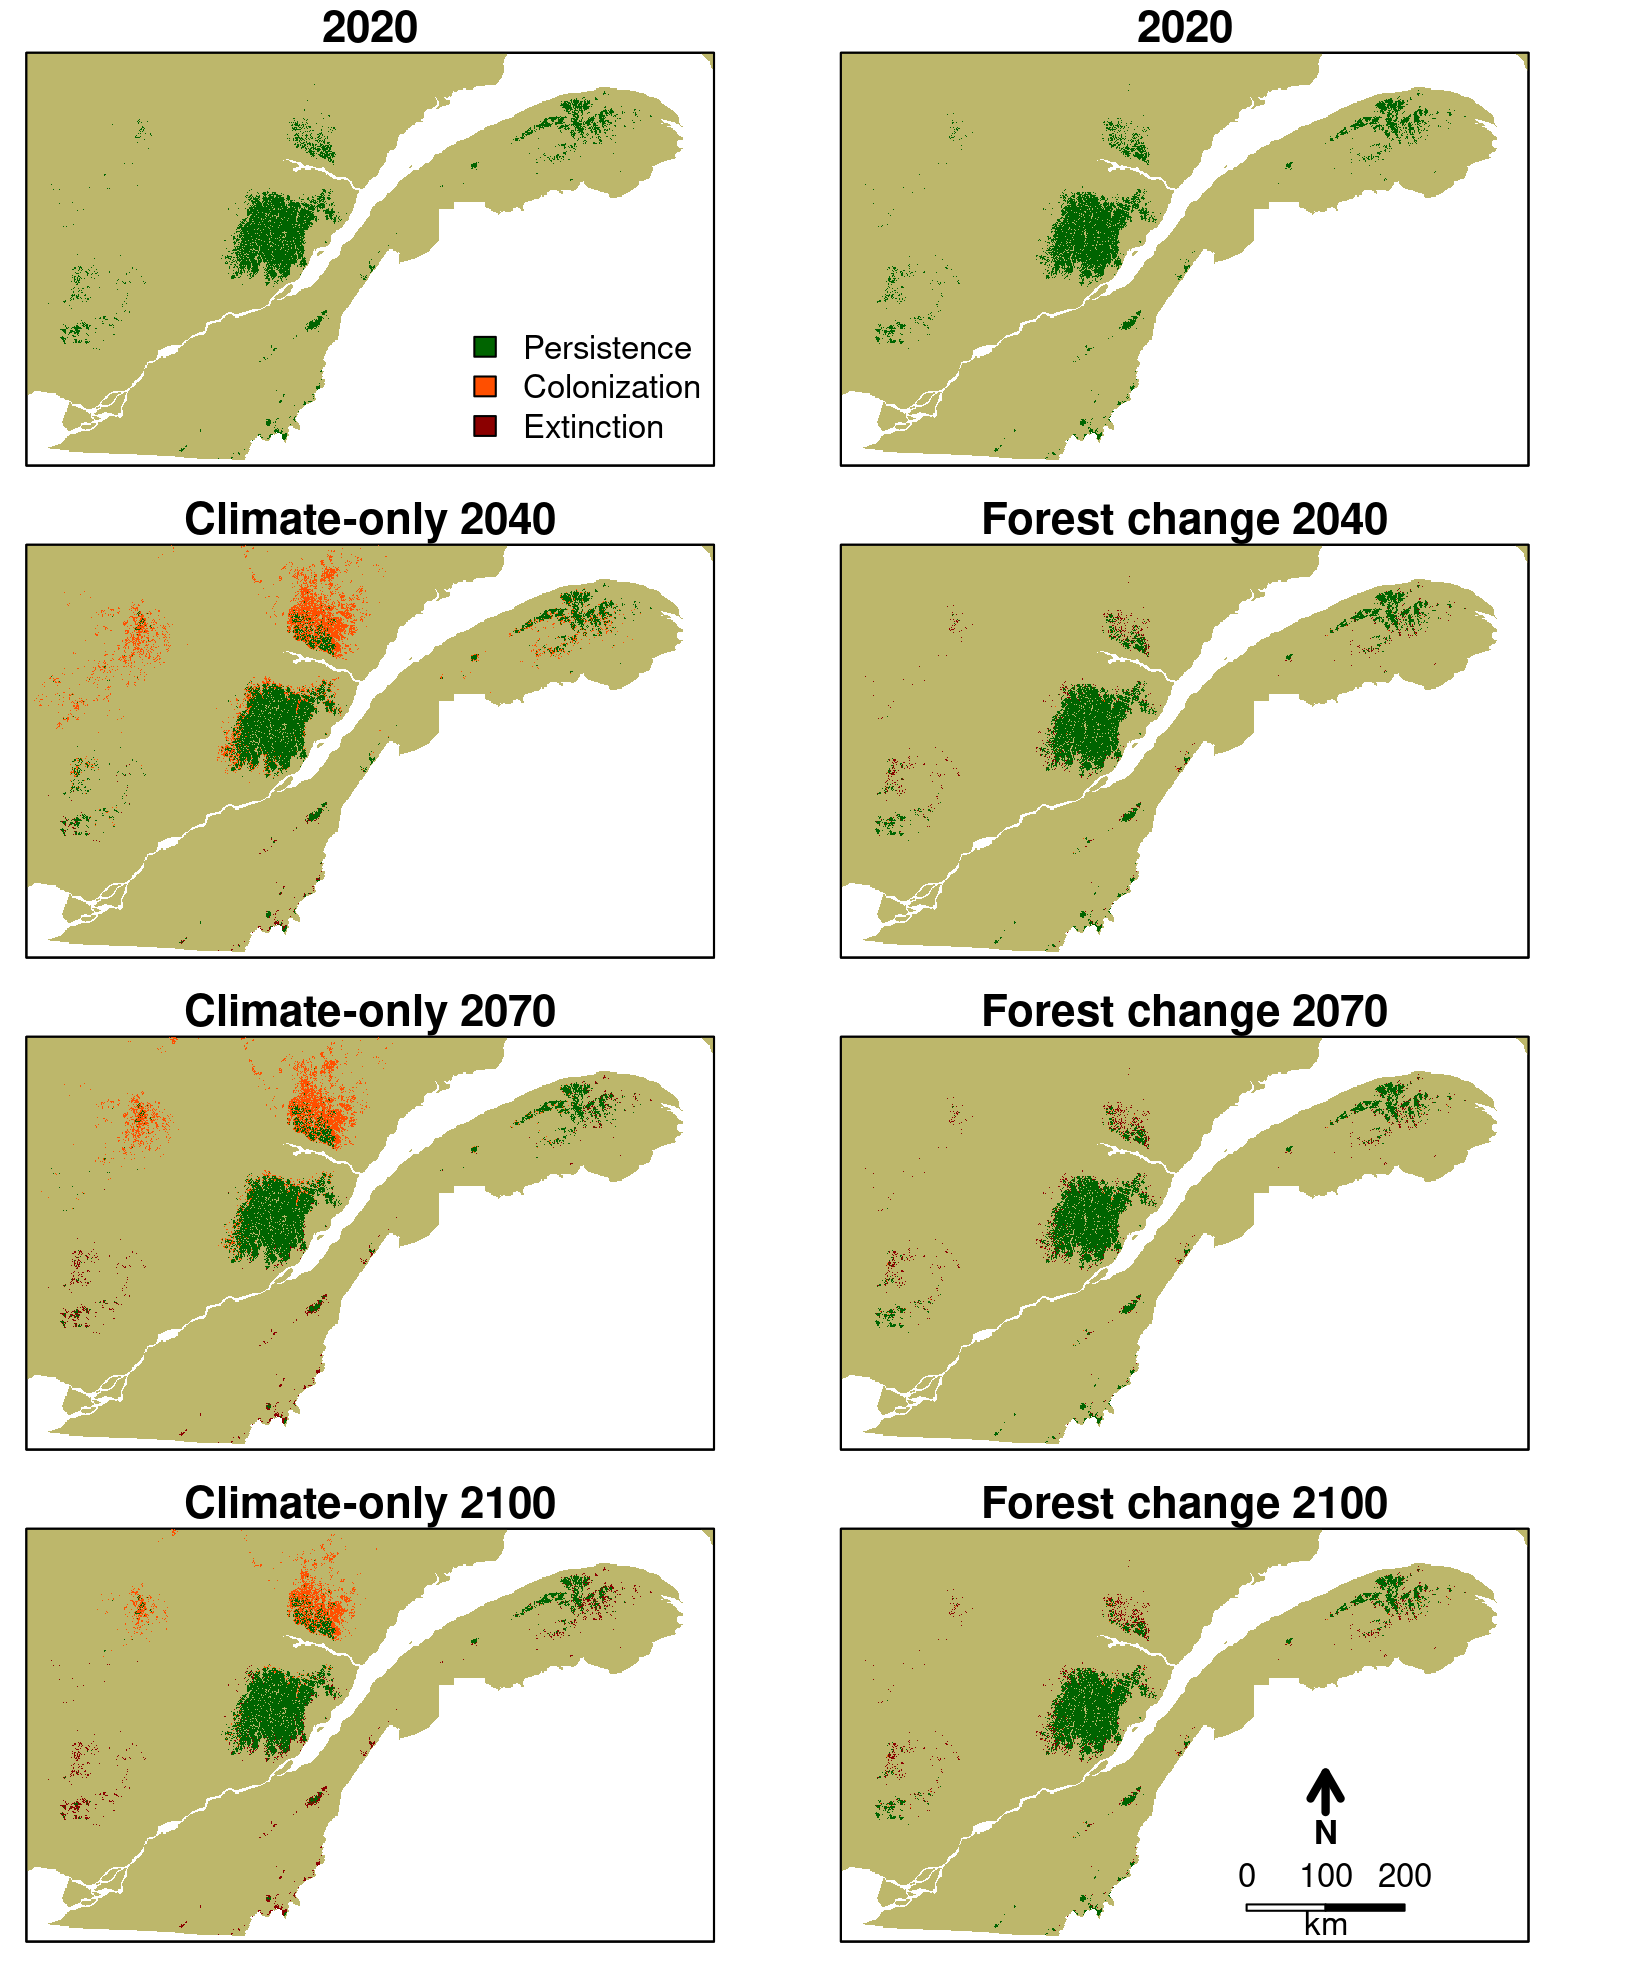
\includegraphics[width=0.8\textwidth,height=\textheight]{./manuscript/img/map_BITH.png}
\caption{Projected Bicknell's thrush breeding range between 2020 and
2100 for climate-only and climate-induced forest change scenarios.
Projected breeding ranges are presented as colonized, persistent, and
extinct patches with 2020 initial distribution as
reference.}\label{fig:map_BITH}
}
\end{figure}

\hypertarget{climate-and-habitat-mismatch}{%
\subsubsection{Climate and habitat
mismatch}\label{climate-and-habitat-mismatch}}

Our model projected varying effects of climate change on Bicknell's
Thrush breeding range within the study region (Figure
\ref{fig:map_BITH}). The magnitude of change differed between
climate-only and climate-induced forest change scenarios. Shifts at the
range edges were more pronounced than within the range under the
climate-only scenario, with contraction at the southern edge and
expansion at the northern edge. Under the climate-only scenario,
extensive expansion was projected as soon as 2040 at high elevation
(\textgreater600 m) and in rapidly warming (up to 3 °C between 2020 and
2040) regions. Multiple northward patches became momentarily suitable
with climate warming at moderate elevation areas (500 to 600 m) because
of the narrow range of suitable climatic conditions at these lower
elevations. Important contraction was projected at the southern range
edge with high elevation mountain tops insufficient to cope with
temperature increase. Conversely, changes in forest composition are
limited due to the slow demography and the limited dispersal of trees
(Vissault et al. \protect\hyperlink{ref-vissault_slow_2020}{2020}). As a
result, the projected changes to the breeding range under the forest
change scenario were much more limited (Figure \ref{fig:map_BITH}).

\hypertarget{changes-in-the-spatial-structure}{%
\subsubsection{Changes in the spatial
structure}\label{changes-in-the-spatial-structure}}

Projections show that climate and forest changes have major consequences
on the spatial structure of suitable patches (Figure
\ref{fig:persistence}, Suppl. Mat. S1). The number of patches within the
breeding range in the climate-only scenario supports the initial
observation of range expansion followed by a rapid contraction with a
peak in number of patches in 2040, while the forest change scenario
shows a decline in number of patches. Overall, median patch area for
both scenarios varied between 0.125 and 0.312 \(km^2\) (minimum and
maximum patch area = 0.0625 and 7805 \(km^2\) respectively) and
indicates a skewed distribution with a dominance of small patches and
few very large ones. On the other hand, the median inter-patch distance
varied between 218 and 280 km (minimum and maximum inter-patch distance
= 0.25 and 809 km respectively) and shows a more balanced distribution
with the landscape composed of distanced groups of regionally close
patches. Although the distribution of patch areas in the climate-only
scenario appears to remain constant through time, important decreases in
the interpatch distances indicate the loss of small, isolated patches,
the addition of geographically close patches, and the fragmentation of
large patches. Despite the apparent stability of the breeding range
under the climate-induced forest change scenario, important changes in
its spatial structure were observed (Figure \ref{fig:persistence}). We
observed a rapid decline in the number of patches and, in contrast to
changes under the climate-only scenario, the median patch area
constantly increased between 2020 and 2100, and the inter-patch distance
marginally increased. Results indicate that close patches became
connected to form fewer, but larger patches in addition to the loss of
small, isolated patches (Suppl. Mat. S1).

\hypertarget{persistence}{%
\subsubsection{Persistence}\label{persistence}}

\begin{figure}
\hypertarget{fig:persistence}{%
\centering
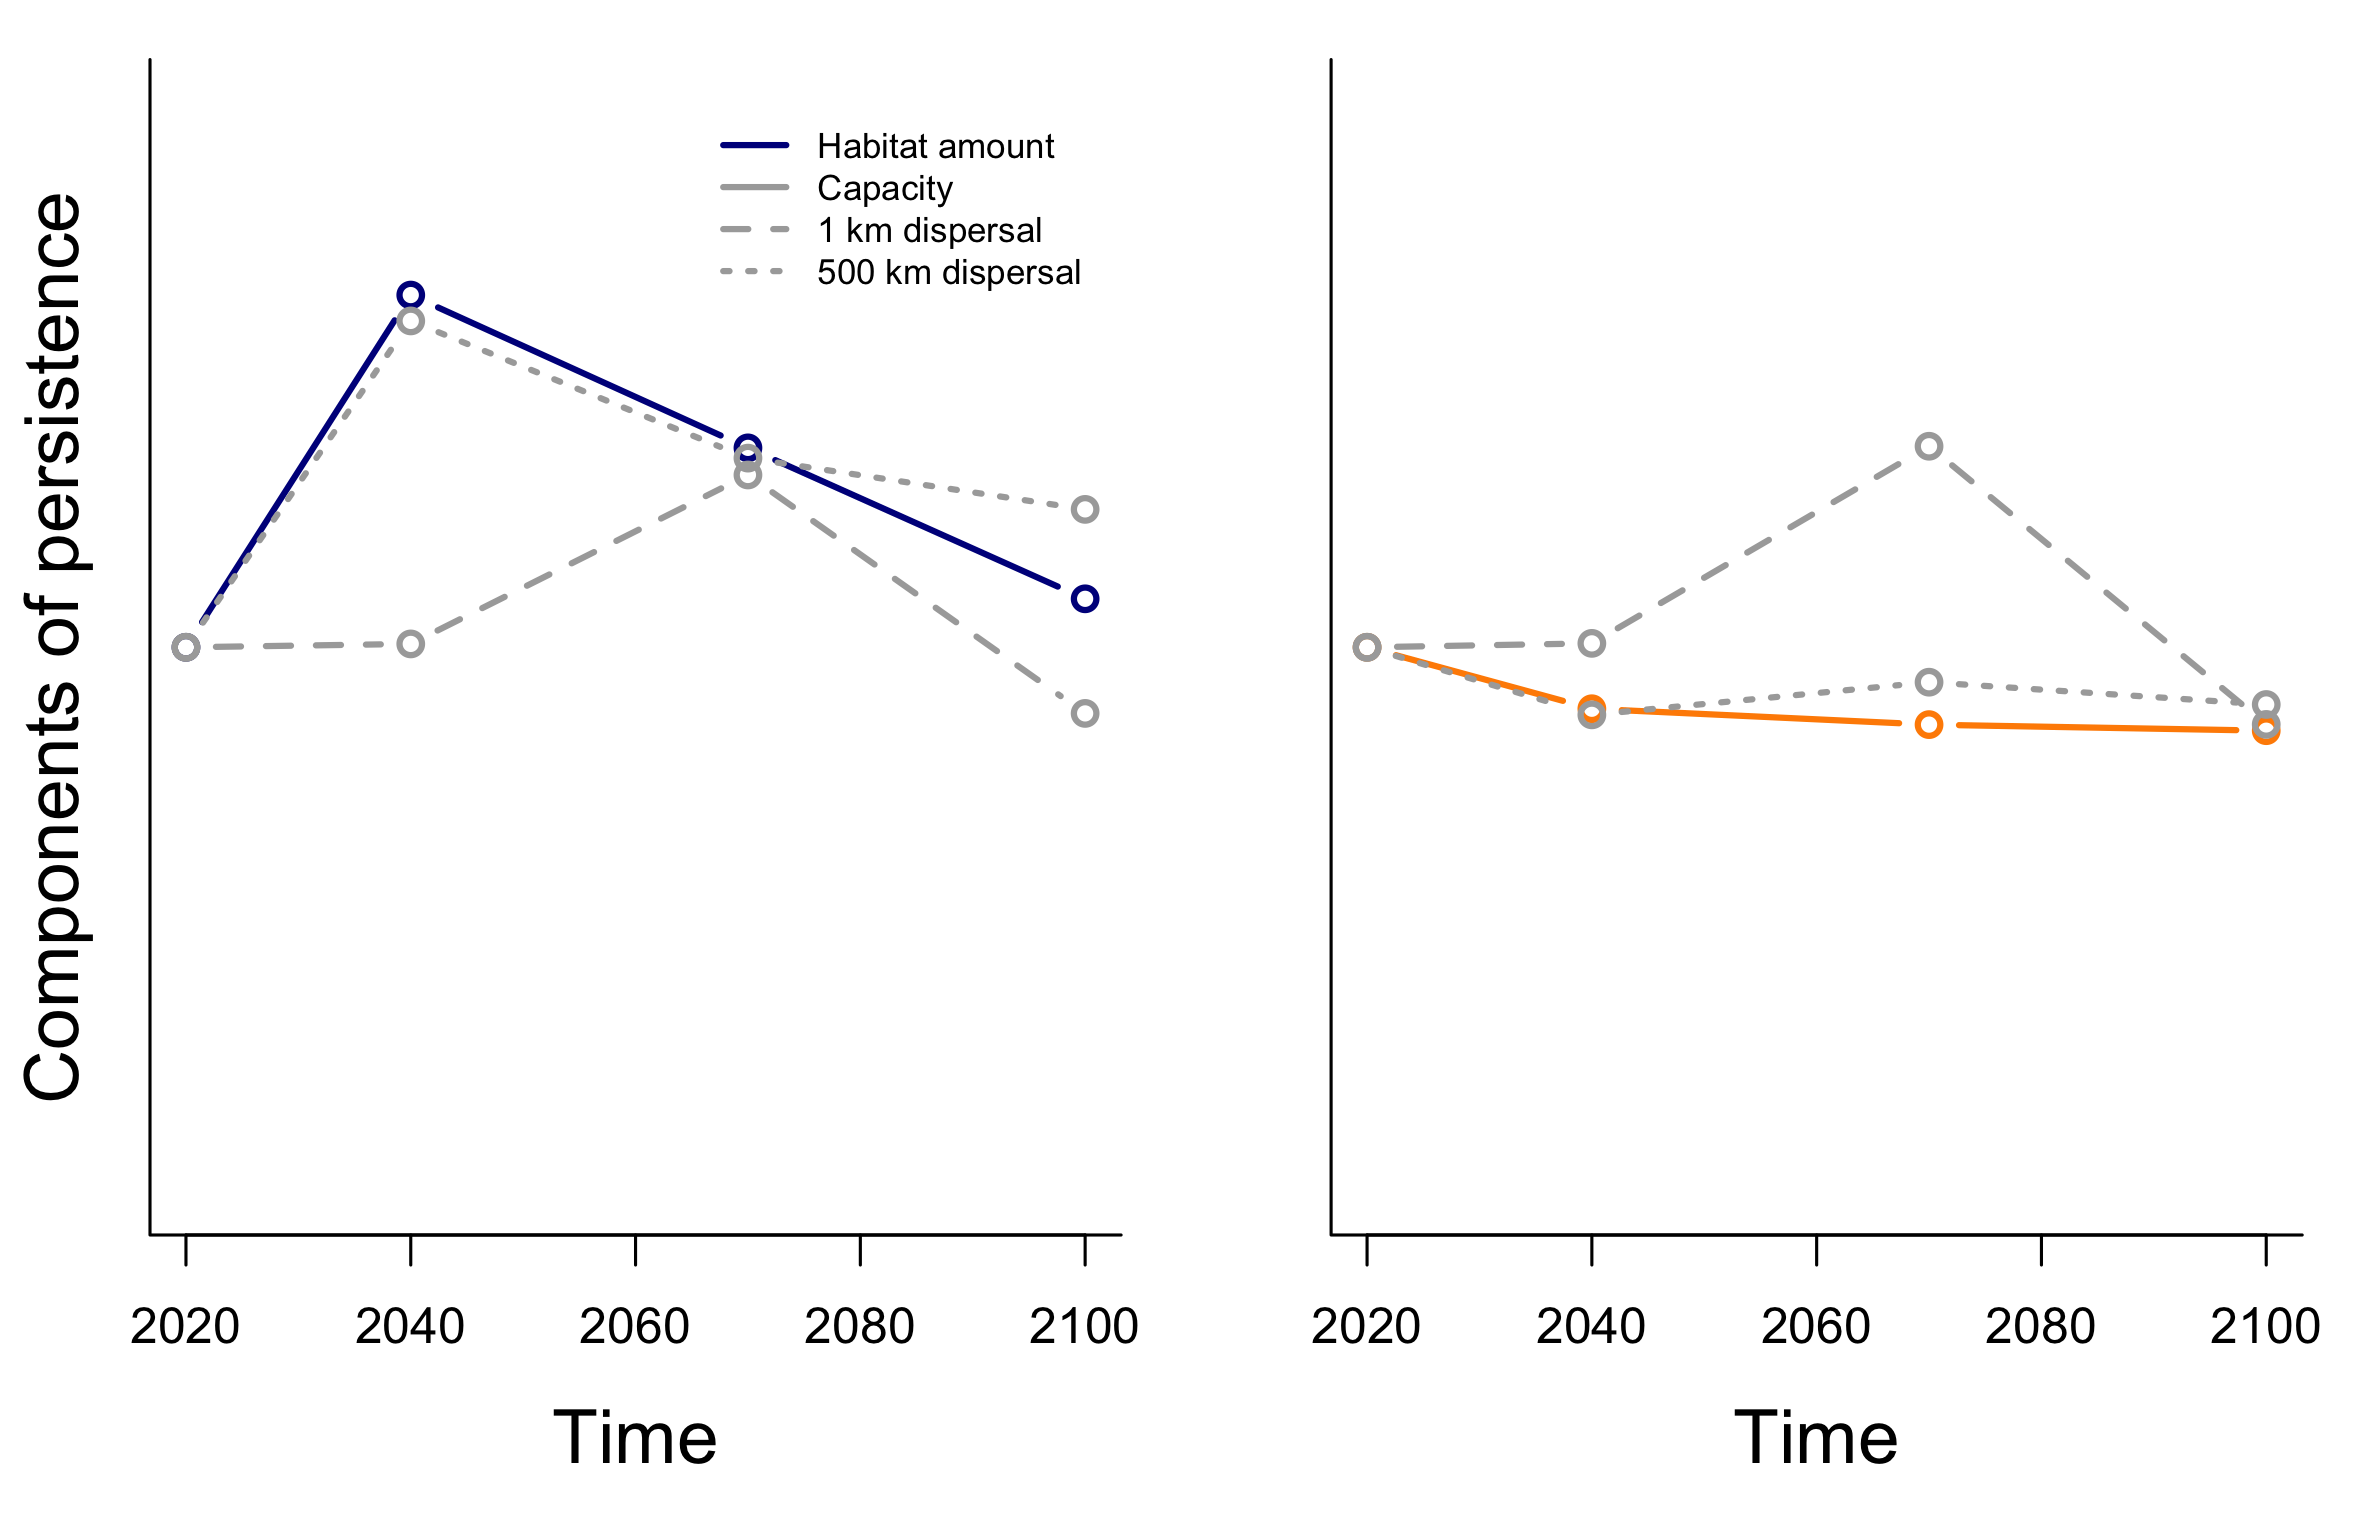
\includegraphics[width=0.75\textwidth,height=\textheight]{./manuscript/img/capacity.png}
\caption{Changes in metrics of metapopulation persistence presented as
metapopulation capacity (dashed lines) and habitat amount (full lines)
from 2020 to 2100. Curves are scaled and centred to the same value in
2020 for comparison. Metapopulation capacity is presented under
restricted dispersal distance (1 km) and an approximation of the mean
field assumption (500 km). Panel A presents climate-only scenario
results and panel B the climate-induced forest change
scenario.}\label{fig:persistence}
}
\end{figure}

We observed an initial increase of 64\% (11,743 to 19,344 \(km^2\)) in
habitat amount under the climate-only scenario (total change of +9\%
between 2020 and 2100; Figure \ref{fig:persistence} A, full blue line)
while habitat amount remained almost stable with only a slight initial
decrease of 11\% (11,742 to 10,416 \(km^2\)) under the climate-induced
forest change scenario (total change of -15\% between 2020 and 2100;
Figure \ref{fig:persistence} B, full orange line). Changes in Bicknell's
Thrush metapopulation capacity approximated those in habitat amount
under long average dispersal distance (approximating mean field
assumption, Figure \ref{fig:persistence}). However, metapopulation
persistence accounting for patch size alone (long-distance dispersal)
was closely approximated by habitat amount but differed when accounting
for both patch size and connectivity (limited dispersal) when changes in
the spatial structure of the breeding range were not explained by
habitat amount alone.

\hypertarget{perspectives}{%
\section{Perspectives}\label{perspectives}}

Using theory and a case study, we show that the climate-induced changes
in distribution are likely to be impacted by bottom-up interactions,
demography, and landscape structure. We first derived three observations
from metapopulation theory. i) A specialist's range is impacted by
changes in habitat occupancy and a habitat-environment mismatch affects
the range limits of the specialist. ii) The interplay between habitat
shrinking and connectivity loss is likely to yield precipitated range
contraction and could potentially lead to extinction. iii) The direction
and amplitude of the specialist's response to environmental change vary
with the degree of environmental response correlation between trophic
levels. We projected the suitable environmental conditions for a
well-known bird species whose distribution is jointly affected by
climate and vegetation and we analyzed its spatial structure. We showed
that climate-induced changes to the distribution of suitable climatic
conditions differed from that of its biotic habitat. Furthermore, both
the amount of habitat and the spatial structure distribution of the
favourable environmental and biotic conditions are predicted to be
impacted by climate change. Thus, we expect the persistence of this
species under climate change to be fundamentally affected by
metapopulation dynamics. We show that the metapopulation approach
complements the understanding of distribution changes by correlative
SDMs. The metapopulation dynamics are fundamental to account for changes
in distributions' spatial structure and contribute to accurately
capturing climate-induced change in species distribution.

\hypertarget{applications-of-the-metapopulation-approach}{%
\subsection{Applications of the metapopulation
approach}\label{applications-of-the-metapopulation-approach}}

Many studies have investigated distribution change using metapopulation
theory (Fordham et al.
\protect\hyperlink{ref-fordham_adapted_2013}{2013}, Huang et al.
\protect\hyperlink{ref-huang_using_2019}{2019}, Schnell et al.
\protect\hyperlink{ref-schnell_estimating_2013}{2013}, Talluto et al.
\protect\hyperlink{ref-talluto_extinction_2017}{2017}, Vissault et al.
\protect\hyperlink{ref-vissault_slow_2020}{2020}), but few have
considered the complexity arising from biotic interactions and dispersal
in context of rapid environmental change. Some aspects have, however,
been explored, starting with the development of the theoretical basis
for metapopulation dynamics on heterogeneous landscapes. Spatially
realistic metapopulation theory has allowed modelling of distribution
dynamics in species living in fragmented landscapes (Hanski
\protect\hyperlink{ref-hanski_metapopulation_1998}{1998},
\protect\hyperlink{ref-hanski_habitat_1999}{1999},
\protect\hyperlink{ref-hanski_spatially_2001}{2001}). The coupling of
spatially explicit metapopulation models with dynamic climate change
represents a significant conceptual advancement toward realistic
projections (Anderson et al.
\protect\hyperlink{ref-anderson_dynamics_2009}{2009}). Our analysis
reveals distribution dynamics that previous methods fail to capture,
demonstrating the importance of integrating dynamic processes. The
metapopulation framework that we propose here proposes to simultaneously
project changes in demography and dispersal in response to climate
change and the multi-species effects of biotic interactions on the
distribution of species.

Metapopulation theory and models influence how conservation priorities
are defined at various scales today. Metapopulation theory predicts the
scaling of extinction risk with increasing habitat isolation, which
non-spatially explicit approaches do not consider. We further show that
a species' ability to access suitable habitat is a determining factor of
its persistence. Assisted colonization and habitat restoration are
proposed as means to support species persistence by increasing
colonization rates and habitat occupancy, respectively (Fordham et al.
\protect\hyperlink{ref-fordham_adapted_2013}{2013}, Ricciardi and
Simberloff \protect\hyperlink{ref-ricciardi_assisted_2009}{2009}, Willis
et al. \protect\hyperlink{ref-willis_assisted_2009}{2009}). Ultimately,
metapopulation theory's main contribution to current conservation
initiatives has been to highlight the effect of landscape spatial
structure and dispersal on species persistence.

\hypertarget{metapopulation-dynamics}{%
\subsection{Metapopulation dynamics}\label{metapopulation-dynamics}}

We have shown using a metapopulation approach that a change in the
occupancy of a habitat along an abiotic environmental gradient may
impact the distribution of higher levels, such as predators or, here,
habitat specialists. Therefore, a mismatch between the distribution of
the habitat and of the favourable environmental conditions may affect
the position of the specialist's range edge along an environmental
gradient. This is the result of local increases or decreases in
colonization and extinction rates from changes in habitat occupancy.
Indeed, we observed the Bicknell's Thrush breeding range projection from
climate-induced forest change to remain stable despite important climate
change. Less contraction than expected from climate-only projections
were observed at the warm edge of southern local habitat patches,
indicating the establishment of a mismatch. The high elevation
coniferous patches persisted into warmer conditions, increasing fir
occupancy under environmental conditions where it was previously rare or
absent. Furthermore, we observed no range expansion of the specialist
where the climate-only scenario predicts northern expansion, revealing a
decrease in habitat occupancy for climatic conditions where it was
previously available. This observation is likely the result of prolonged
persistence (i.e., extinction debt) of the Bicknell's Thrush where it is
already observed despite less favourable environmental conditions, and
the reduction of occupancy in favourable environmental conditions where
it is initially observed (i.e., colonization credit). As a result,
non-equilibrium dynamics in Bicknell's Thrush distribution change are
predicted to be an important source of complexity. Forested
habitat-environment, or resource-environment mismatch in response to
environmental change is to be expected in natural systems from
limitations in dispersal ability and demography (Svenning et al.
\protect\hyperlink{ref-svenning_influence_2014}{2014}). Conversely,
habitats that shift faster than abiotic environmental conditions may
instead decrease specialist persistence in its current range and favour
environmental, but not geographical range stability. It is clear that
non-equilibrium dynamics in species distributions are key elements of
complexity. Hence, predictions are likely to be biased without proper
models to account for it.

Correlative SDMs predict direct response of species' range to habitat
amount variations such that a decrease in habitat amount causes an
equivalent contraction of the species' range. However, we have shown
that a metapopulation framework offers complementary information to
extract from habitat projections. The contraction of a species' range
may be accelerated (or slowed) by metapopulation dynamics. Here, the
effect of landscape connectivity interacts with habitat occupancy to
generate dynamics of greater complexity. We observed changes in the
Bicknell's Thrush distribution projections in both habitat amount and in
spatial structure of habitat patches. Landscape connectivity was
affected by newly suitable habitat patches, the extinction of the
smallest habitat patches, the fragmentation of the larger ones, and the
dispersal distance. In concordance with our intuition, changes in
Bicknell's Thrush persistence were affected by metapopulation dynamics.
Persistence could not be explained by changes in habitat amount alone
contrasting with the assumption made by correlative SDMs (Figure
\ref{fig:persistence}). Furthermore, our results support Hanski
(\protect\hyperlink{ref-hanski_habitat_2015}{2015}) in that connectivity
is fundamental to species regional distribution, abundance, and
biodiversity in opposition to the habitat amount hypothesis (Fahrig
\protect\hyperlink{ref-fahrig_rethinking_2013}{2013}). That is because
the species' ability to use all available habitat is affected by
dispersal, which habitat amount alone does not represent.

More favourable abiotic environmental conditions can have unexpected
negative impacts on specialists if their habitats are negatively
affected. We described this phenomenon as the effect of environmental
response correlation between trophic levels (see \emph{Key concepts}
section). It is a concept unique to process-based approaches that cannot
be observed directly using a correlative SDM approach as it originates
from the joint effects of species-specific environmental performance and
of biotic interactions. Although we have not been able to measure it
directly with the Bicknell's Thrush case, we observed an important
contrast between its response to climate-only change and to
climate-induced forest change: the habitat amount increased in the first
scenario and declined in the second. We showed that regionally more
favourable climatic conditions to the Bicknell's Thrush may have, even
if only temporarily due to colonization or extinction lags, the opposite
effect on its habitat. Therefore, the resulting distribution dynamics
from the interplay between trophic levels are complex to predict.
Counterintuitive dynamics can arise from species' environmental
correlation. Indeed, the Bicknell's thrush example illustrates the
necessity of documenting the response between trophic levels to a
rapidly changing environment as they can produce non-equilibrium
dynamics when considered together. It is when the lower trophic level
affects the specialist's colonization and extinction rates
asymmetrically that non-equilibrium distribution dynamics are observed.
Because metapopulation models can incorporate such dynamics on
specialists' population dynamics, the resulting projections may be of
greater realism.

\hypertarget{limitations-of-the-current-approach}{%
\subsection{Limitations of the current
approach}\label{limitations-of-the-current-approach}}

Metapopulation models require few parameters making them relatively easy
to parameterize. Even in the absence of a calibrated model, the
metapopulation approach offers tools to interpret projections outputs
from correlative SDMs. We showed that different aspects of the
landscape's structure could easily be described and studied. An
integrated interpretation of distribution changes can be gained from
scenarios of dispersal and extinction. Such scenarios can then be used
to evaluate species persistence.

Several other factors could also impact the system's response to climate
warming. The model described here is best suited for habitat specialists
whose presence depends on the prior establishment of another species
that they do not impact, but it could also be generalized to other types
of interactions (Gravel et al.
\protect\hyperlink{ref-gravel_trophic_2011}{2011}). The concepts
developed in this study are more general than the specialist-habitat
context in which they are presented and can apply to any bottom-up
system. Positive and negative effects of the specialist on its habitat
could influence the system's response to climate change differently. For
example, habitat (i.e., resource) removal by the specialist may reduce
competition of habitat types and decrease response lag, accelerating the
specialist's decline at the scale of the landscape (Vissault et al.
\protect\hyperlink{ref-vissault_slow_2020}{2020}). Prolonged occupancy
of the habitat by the specialist may, on the other hand, increase
habitat mismatch and support source-sink dynamics (Pulliam
\protect\hyperlink{ref-pulliam_sources_1988}{1988}). In addition to
biotic interactions, metapopulation dynamics at the landscape level
could be affected by the interaction of climate change and natural
disturbances. For instance, wildfires and insect outbreak regimes are
expected to be strongly altered under climate change (Boulanger and
Pascual Puigdevall \protect\hyperlink{ref-boulanger_boreal_2021}{2021}),
and associated biodiversity (see Tremblay et al.
(\protect\hyperlink{ref-tremblay_harvesting_2018}{2018}) for a case
study). Both are important drivers of forest dynamics, and our results
show that modification in habitat distribution is associated with the
specialist response.

We hope that biodiversity actors benefit from more accurate, yet
accessible methods to estimate distribution changes. Correlative SDMs
are most often used to project distribution changes, but metapopulation
models allow a more accurate estimation of colonization and extinction
rates with a multispecies perspective. Our estimation of the Bicknell's
Thrush range projected that the biotic interactions will favour the
species' persistence where it already occurs, but will limit its
progression further north where firs are not as abundant despite
increases in climate suitability. The resulting effect is likely to be
the regional contraction of the Bicknell's Thrush range despite more
favourable climatic conditions. Our study highlights the importance of
demography, dispersal and biotic interactions on distribution change to
rapid environmental change and the importance of spatial structure on
the interpretation of projections.

\newpage

\hypertarget{references}{%
\section*{References}\label{references}}
\addcontentsline{toc}{section}{References}

\hypertarget{refs}{}
\begin{cslreferences}
\leavevmode\hypertarget{ref-anderson_dynamics_2009}{}%
Anderson, B. J., H. R. Akçakaya, M. B. Ara\a'ujo, D. A. Fordham, E.
Martinez-Meyer, W. Thuiller, and B. W. Brook. 2009. Dynamics of range
margins for metapopulations under climate change. Proceedings of the
Royal Society B: Biological Sciences 276:1415--1420.

\leavevmode\hypertarget{ref-boulangeat_transient_2018}{}%
Boulangeat, I., J. C. Svenning, T. Daufresne, M. Leblond, and D. Gravel.
2018. The transient response of ecosystems to climate change is
amplified by trophic interactions. Oikos 127:1822--1833.

\leavevmode\hypertarget{ref-boulanger_boreal_2021}{}%
Boulanger, Y., and J. Pascual Puigdevall. 2021. Boreal forests will be
more severely affected by projected anthropogenic climate forcing than
mixedwood and northern hardwood forests in eastern Canada. Landscape
Ecology 36:1725--1740.

\leavevmode\hypertarget{ref-briscoe_can_2021}{}%
Briscoe, N. J., D. Zurell, J. Elith, C. König, G. Fandos, A. Malchow, M.
K\a'ery, H. Schmid, and G. GuillerNAaNAArroi. 2021. Can dynamic
occupancy models improve predictions of species' range dynamics? A test
using Swiss birds. Global Change Biology 27:4269--4282.

\leavevmode\hypertarget{ref-cadieux_spatially_2019}{}%
Cadieux, P., Y. Boulanger, D. Cyr, A. R. Taylor, D. T. Price, and J. A.
Tremblay. 2019. Spatially explicit climate change projections for the
recovery planning of threatened species: The Bicknell's Thrush (Catharus
Bicknelli) as a case study. Global Ecology and Conservation 17:e00530.

\leavevmode\hypertarget{ref-chen_rapid_2011}{}%
Chen, I. C., J. K. Hill, R. Ohlemüller, D. B. Roy, and C. D. Thomas.
2011. Rapid range shifts of species associated with high levels of
climate warming. Science 333:1024--1026.

\leavevmode\hypertarget{ref-collins_spatial_2007}{}%
Collins, B. B. 2007. Spatial Analysis of Home Range, Movement Patterns,
and Behavioral Ecology of Bicknell's Thrush, Catharus bicknelli, in
Vermont. Master's thesis, Antioch University, Antioch University, Keene
(New Hampshire).

\leavevmode\hypertarget{ref-cosewic_cosewic_2022}{}%
COSEWIC. 2022. COSEWIC assessment and status report on the Bicknell's
Thrush Catharus bicknelli in canada. Page 64. Committee on the Status of
Endangered Wildlife in Canada, Ottawa.

\leavevmode\hypertarget{ref-fahrig_rethinking_2013}{}%
Fahrig, L. 2013. Rethinking patch size and isolation effects: The
habitat amount hypothesis. Journal of Biogeography 40:1649--1663.

\leavevmode\hypertarget{ref-fordham_adapted_2013}{}%
Fordham, D. A., H. R. Akçakaya, B. W. Brook, A. Rodr\a'ıguez, P. C.
Alves, E. Civantos, M. Triviño, M. J. Watts, and M. B. Ara\a'ujo. 2013.
Adapted conservation measures are required to save the Iberian lynx in a
changing climate. Nature Climate Change 3:899--903.

\leavevmode\hypertarget{ref-franklin_mapping_2009}{}%
Franklin, J., and J. A. Miller. 2009. Mapping species distributions:
Spatial inference and prediction. Cambridge University Press, Cambridge
; New York.

\leavevmode\hypertarget{ref-godsoe_integrating_2017}{}%
Godsoe, W., J. Jankowski, R. D. Holt, and D. Gravel. 2017. Integrating
Biogeography with Contemporary Niche Theory. Trends in Ecology and
Evolution 32:488--499.

\leavevmode\hypertarget{ref-gravel_trophic_2011}{}%
Gravel, D., F. Massol, E. Canard, D. Mouillot, and N. Mouquet. 2011.
Trophic theory of island biogeography. Ecology Letters 14:1010--1016.

\leavevmode\hypertarget{ref-guisan_predicting_2005}{}%
Guisan, A., and W. Thuiller. 2005. Predicting species distribution:
Offering more than simple habitat models. Ecology Letters 8:993--1009.

\leavevmode\hypertarget{ref-guisan_predicting_2013}{}%
Guisan, A., R. Tingley, J. B. Baumgartner, I. NaujokaitisNANALewis, P.
R. Sutcliffe, A. I. T. Tulloch, T. J. Regan, L. Brotons, E.
McDonalNAdNAMadden, C. MantyNAkaNAPringle, T. G. Martin, J. R. Rhodes,
R. Maggini, S. A. Setterfield, J. Elith, M. W. Schwartz, B. A. Wintle,
O. Broennimann, M. Austin, S. Ferrier, M. R. Kearney, H. P. Possingham,
and Y. M. Buck. 2013. Predicting species distributions for conservation
decisions. Ecology Letters 16:1424--1435.

\leavevmode\hypertarget{ref-hanski_metapopulation_1998}{}%
Hanski, I. 1998. Metapopulation dynamics. Nature 396:41--49.

\leavevmode\hypertarget{ref-hanski_habitat_1999}{}%
Hanski, I. 1999. Habitat Connectivity , Habitat Continuity , and
Metapopulations in Dynamic Landscapes. Oikos, Nordic Society
87:209--219.

\leavevmode\hypertarget{ref-hanski_spatially_2001}{}%
Hanski, I. 2001. Spatially realistic theory of metapopulation ecology.
Naturwissenschaften 88:372--381.

\leavevmode\hypertarget{ref-hanski_habitat_2015}{}%
Hanski, I. 2015. Habitat fragmentation and species richness. Journal of
Biogeography 42:989--993.

\leavevmode\hypertarget{ref-hanski_metapopulation_2000}{}%
Hanski, I., and O. Ovaskainen. 2000. The metapopulation capacity of a
fragmented landscape. Nature 404:755--758.

\leavevmode\hypertarget{ref-hanski_metapopulation_1997}{}%
Hanski, I., and D. Simberloff. 1997. The Metapopulation Approach, Its
History, Conceptual Domain, and Application to Conservation. Pages 5--26
\emph{in} I. Hanski and M. E. Gilpin, editors. Metapopulation Biology.
Academic Press, San Diego.

\leavevmode\hypertarget{ref-hausfather_emissions_2020}{}%
Hausfather, Z., and G. P. Peters. 2020. Emissions -- the ``business as
usual'' story is misleading. Nature 577:618--620.

\leavevmode\hypertarget{ref-hefley_when_2017}{}%
Hefley, T. J., M. B. Hooten, R. E. Russell, D. P. Walsh, and J. A.
Powell. 2017. When mechanism matters: Bayesian forecasting using models
of ecological diffusion. Ecology Letters 20:640--650.

\leavevmode\hypertarget{ref-hollister_elevatr_2021}{}%
Hollister, J. W., A. L. Robitaille, M. W. Beck, MikeJohnson-NOAA, and T.
Shah. 2021, July. Elevatr: Access elevation data from various APIs.
Zenodo.

\leavevmode\hypertarget{ref-huang_using_2019}{}%
Huang, R., S. L. Pimm, and C. Giri. 2019. Using metapopulation theory
for practical conservation of mangrove endemic birds. Conservation
Biology 34:266--275.

\leavevmode\hypertarget{ref-hutchinson_concluding_1957}{}%
Hutchinson, G. E. 1957. Concluding remarks. Cold spring harbor symposia
on quantitative biology 22:415--427.

\leavevmode\hypertarget{ref-iucn_catharus_2020}{}%
IUCN. 2020, August. Catharus bicknelli: BirdLife International: The IUCN
Red List of Threatened Species 2020: E.T22728467A180783383.

\leavevmode\hypertarget{ref-le_squin_climateinduced_2021}{}%
Le Squin, A., I. Boulangeat, and D. Gravel. 2021. Climate‐induced
variation in the demography of 14 tree species is not sufficient to
explain their distribution in eastern North America. Global Ecology and
Biogeography 30:352--369.

\leavevmode\hypertarget{ref-levins_demographic_1969}{}%
Levins, R. 1969. Some demographic and genetic consequences of
environmental heterogeneity for biological control. Bulletin of the
Entomological Society of America 15:237--240.

\leavevmode\hypertarget{ref-levins_mathematical_1970}{}%
Levins, R. 1970. Some Mathematical Questions in Biology. \emph{in} Some
Mathematical Questions in Biology.

\leavevmode\hypertarget{ref-mcgill_trees_2012}{}%
McGill, B. J. 2012. Trees are rarely most abundant where they grow best.
Journal of Plant Ecology 5:46--51.

\leavevmode\hypertarget{ref-mcintire_perfict_2022}{}%
McIntire, E. J. B., A. M. Chubaty, S. G. Cumming, D. Andison, C. Barros,
C. Boisvenue, S. Hach\a'e, Y. Luo, T. Micheletti, and F. E. C. Stewart.
2022. PERFICT: A Re‐imagined foundation for predictive ecology. Ecology
Letters 25:1345--1351.

\leavevmode\hypertarget{ref-mckenney_spatial_2013}{}%
McKenney, D., J. Pedlar, M. Hutchinson, P. Papadopol, K. Lawrence, K.
Campbell, E. Milewska, R. F. Hopkinson, and D. Price. 2013. Spatial
climate models for Canada's forestry community. The Forestry Chronicle
89:659--663.

\leavevmode\hypertarget{ref-mckenney_customized_2011}{}%
McKenney, D. W., M. F. Hutchinson, P. Papadopol, K. Lawrence, J. Pedlar,
K. Campbell, E. Milewska, R. F. Hopkinson, D. Price, and T. Owen. 2011.
Customized Spatial Climate Models for North America. Bulletin of the
American Meteorological Society 92:1611--1622.

\leavevmode\hypertarget{ref-ovaskainen_transient_2002}{}%
Ovaskainen, O., and I. Hanski. 2002. Transient Dynamics in
Metapopulation Response to Perturbation. Theoretical Population Biology
61:285--295.

\leavevmode\hypertarget{ref-parmesan_ecological_2006}{}%
Parmesan, C. 2006. Ecological and Evolutionary Responses to Recent
Climate Change. Annual Review of Ecology, Evolution, and Systematics
37:637--669.

\leavevmode\hypertarget{ref-pulliam_sources_1988}{}%
Pulliam, H. R. 1988. Sources, Sinks, and Population Regulation. The
American Naturalist 132:652--661.

\leavevmode\hypertarget{ref-regniere_biosim_2017}{}%
R\a'egni\a`ere, J., R. Saint-Amant, A. B\a'echard, and A. Moutaoufik.
2017. BioSIM 11 user's manual. Natural Resources Canada, Canadian Forest
Services, Laurentian Forestry Center, Québec, Canada.

\leavevmode\hypertarget{ref-regniere_stochastic_2007}{}%
R\a'egni\a`ere, J., and R. St-Amant. 2007. Stochastic simulation of
daily air temperature and precipitation from monthly normals in North
America north of Mexico. International Journal of Biometeorology
51:415--430.

\leavevmode\hypertarget{ref-renner_point_2015}{}%
Renner, I. W., J. Elith, A. Baddeley, W. Fithian, T. Hastie, S. J.
Phillips, G. Popovic, and D. I. Warton. 2015. Point process models for
presence‐only analysis. Methods in Ecology and Evolution 6:366--379.

\leavevmode\hypertarget{ref-ricciardi_assisted_2009}{}%
Ricciardi, A., and D. Simberloff. 2009. Assisted colonization is not a
viable conservation strategy. Trends in Ecology \& Evolution
24:248--253.

\leavevmode\hypertarget{ref-rimmer_bicknells_2001}{}%
Rimmer, C. C., J. D. Lambert, K. P. Mcfarl, and D. Busby. 2001.
Bicknell's Thrush: Catharus bicknelli. \emph{in} The birds of North
America, 592. The Birds of North. America, Inc.

\leavevmode\hypertarget{ref-robin_proc_2011}{}%
Robin, X., N. Turck, A. Hainard, F. Lisacek, and J.-C. Sanchez. 2011.
pROC: An open-source package for R and S+ to analyze and compare ROC
curves. BMC Bioinformatics 12:1--8.

\leavevmode\hypertarget{ref-rodenhouse_potential_2008}{}%
Rodenhouse, N. L., S. N. Matthews, K. P. McFarland, J. D. Lambert, L. R.
Iverson, A. Prasad, T. S. Sillett, and R. T. Holmes. 2008. Potential
effects of climate change on birds of the Northeast. Mitigation and
Adaptation Strategies for Global Change 13:517--540.

\leavevmode\hypertarget{ref-savage_elevational_2015}{}%
Savage, J., and M. Vellend. 2015. Elevational shifts, biotic
homogenization and time lags in vegetation change during 40 years of
climate warming. Ecography 38:546--555.

\leavevmode\hypertarget{ref-scheller_design_2007}{}%
Scheller, R. M., J. B. Domingo, B. R. Sturtevant, J. S. Williams, A.
Rudy, E. J. Gustafson, and D. J. Mladenoff. 2007. Design, development,
and application of LANDIS-II, a spatial landscape simulation model with
flexible temporal and spatial resolution. Ecological Modelling
201:409--419.

\leavevmode\hypertarget{ref-schnell_estimating_2013}{}%
Schnell, J. K., G. M. Harris, S. L. Pimm, and G. J. Russell. 2013.
Estimating Extinction Risk with Metapopulation Models of Large-Scale
Fragmentation. Conservation Biology 27:520--530.

\leavevmode\hypertarget{ref-snell_using_2014}{}%
Snell, R. S., A. Huth, J. E. M. S. Nabel, G. Bocedi, J. M. J. Travis, D.
Gravel, H. Bugmann, A. G. Guti\a'errez, T. Hickler, S. I. Higgins, B.
Reineking, M. Scherstjanoi, N. Zurbriggen, and H. Lischke. 2014. Using
dynamic vegetation models to simulate plant range shifts. Ecography
37:1184--1197.

\leavevmode\hypertarget{ref-sos-pop_banque_2021}{}%
SOS-POP. 2021. Banque de données sur les populations d'oiseaux en
situation précaire au Québec. Données issues du programme de Suivi des
sites importants pour la conservation des populations d'oiseaux en péril
du Québec. QuébecOiseaux, Montréal, Québec.

\leavevmode\hypertarget{ref-stephan_positive_2021}{}%
Stephan, P., B. B. Mora, and J. M. Alexander. 2021. Positive species
interactions shape species' range limits. Oikos:1611--1625.

\leavevmode\hypertarget{ref-stralberg_conservation_2015}{}%
Stralberg, D., E. M. Bayne, S. G. Cumming, P. S\a'olymos, S. J. Song,
and F. K. A. Schmiegelow. 2015. Conservation of future boreal forest
bird communities considering lags in vegetation response to climate
change: A modified refugia approach. Diversity and Distributions
21:1112--1128.

\leavevmode\hypertarget{ref-stralberg_conservation_2019}{}%
Stralberg, D., D. Berteaux, C. R. Drever, M. Drever, I.
Naujokaitis-Lewis, F. K. A. Schmiegelow, and J. A. Tremblay. 2019.
Conservation planning for boreal birds in a changing climate: A
framework for action. Avian Conservation and Ecology 14:art13.

\leavevmode\hypertarget{ref-studds_stable-hydrogen_2012}{}%
Studds, C. E., K. P. McFarland, Y. Aubry, C. C. Rimmer, K. A. Hobson, P.
P. Marra, and L. I. Wassenaar. 2012. Stable-hydrogen isotope measures of
natal dispersal reflect observed population declines in a threatened
migratory songbird. Diversity and Distributions 18:919--930.

\leavevmode\hypertarget{ref-svenning_influence_2014}{}%
Svenning, J. C., D. Gravel, R. D. Holt, F. M. Schurr, W. Thuiller, T.
Münkemüller, K. H. Schiffers, S. Dullinger, T. C. Edwards, T. Hickler,
S. I. Higgins, J. E. M. S. Nabel, J. Pagel, and S. Normand. 2014. The
influence of interspecific interactions on species range expansion
rates. Ecography 37:1198--1209.

\leavevmode\hypertarget{ref-svenning_disequilibrium_2013}{}%
Svenning, J. C., and B. Sandel. 2013. Disequilibrium vegetation dynamics
under future climate change. American Journal of Botany 100:1266--1286.

\leavevmode\hypertarget{ref-talluto_extinction_2017}{}%
Talluto, M. V., I. Boulangeat, S. Vissault, W. Thuiller, and D. Gravel.
2017. Extinction debt and colonization credit delay range shifts of
eastern North American trees. Nature Ecology \& Evolution 1:0182--0182.

\leavevmode\hypertarget{ref-thomas_extinction_2004}{}%
Thomas, C. D., A. Cameron, G. F. Midgley, A. T. Peterson, S. E.
Williams, A. Cameron, R. E. Green, and M. Bakkenes. 2004. Extinction
risk from climate change. Nature 427:145--148.

\leavevmode\hypertarget{ref-thuiller_road_2013}{}%
Thuiller, W., T. Münkemüller, S. Lavergne, D. Mouillot, N. Mouquet, K.
Schiffers, and D. Gravel. 2013. A road map for integrating
eco-evolutionary processes into biodiversity models. Ecology Letters
16:94--105.

\leavevmode\hypertarget{ref-billerman_bicknells_2020}{}%
Townsend, J. M., K. P. McFarland, C. C. Rimmer, W. G. Ellison, and J. E.
Goetz. 2020. Bicknell's Thrush (Catharus bicknelli). \emph{in} S. M.
Billerman, B. K. Keeney, P. G. Rodewald, and T. S. Schulenberg, editors.
Birds of the World. Cornell Lab of Ornithology.

\leavevmode\hypertarget{ref-tremblay_harvesting_2018}{}%
Tremblay, J. A., Y. Boulanger, D. Cyr, A. R. Taylor, D. T. Price, and
M.-H. St-Laurent. 2018. Harvesting interacts with climate change to
affect future habitat quality of a focal species in eastern Canada's
boreal forest. PLOS ONE 13:e0191645.

\leavevmode\hypertarget{ref-urban_improving_2016}{}%
Urban, M. C., G. Bocedi, A. P. Hendry, J. B. Mihoub, G. Pe'er, A.
Singer, J. R. Bridle, L. G. Crozier, L. De Meester, W. Godsoe, A.
Gonzalez, J. J. Hellmann, R. D. Holt, A. Huth, K. Johst, C. B. Krug, P.
W. Leadley, S. C. F. Palmer, J. H. Pantel, A. Schmitz, P. A. Zollner,
and J. M. J. Travis. 2016. Improving the forecast for biodiversity under
climate change. Science 353:aad8466.

\leavevmode\hypertarget{ref-van_vuuren_representative_2011}{}%
van Vuuren, D. P., J. Edmonds, M. Kainuma, K. Riahi, A. Thomson, K.
Hibbard, G. C. Hurtt, T. Kram, V. Krey, J.-F. Lamarque, T. Masui, M.
Meinshausen, N. Nakicenovic, S. J. Smith, and S. K. Rose. 2011. The
representative concentration pathways: An overview. Climatic Change
109:5--31.

\leavevmode\hypertarget{ref-virkkala_patterns_2014}{}%
Virkkala, R., and A. Lehikoinen. 2014. Patterns of climate-induced
density shifts of species: Poleward shifts faster in northern boreal
birds than in southern birds. Global Change Biology 20:2995--3003.

\leavevmode\hypertarget{ref-vissault_slow_2020}{}%
Vissault, S., M. V. Talluto, I. Boulangeat, and D. Gravel. 2020. Slow
demography and limited dispersal constrain the expansion of
north-eastern temperate forests under climate change. Journal of
Biogeography 47:2645--2656.

\leavevmode\hypertarget{ref-willis_assisted_2009}{}%
Willis, S. G., J. K. Hill, C. D. Thomas, D. B. Roy, R. Fox, D. S.
Blakeley, and B. Huntley. 2009. Assisted colonization in a changing
climate: A test-study using two U.K. Butterflies. Conservation Letters
2:46--52.
\end{cslreferences}


\newpage


\end{document}